%% 
%% Copyright 2019-2021 Elsevier Ltd
%% 
%% This file is part of the 'CAS Bundle'.
%% --------------------------------------
%% 
%% It may be distributed under the conditions of the LaTeX Project Public
%% License, either version 1.2 of this license or (at your option) any
%% later version.  The latest version of this license is in
%%    http://www.latex-project.org/lppl.txt
%% and version 1.2 or later is part of all distributions of LaTeX
%% version 1999/12/01 or later.
%% 
%% The list of all files belonging to the 'CAS Bundle' is
%% given in the file `manifest.txt'.
%% 
%% Template article for cas-dc documentclass for 
%% double column output.

\documentclass[a4paper,fleqn]{cas-dc}

% If the frontmatter runs over more than one page
% use the longmktitle option.

%\documentclass[a4paper,fleqn,longmktitle]{cas-dc}

%\usepackage[numbers]{natbib}
%\usepackage[authoryear]{natbib}
\usepackage[authoryear,longnamesfirst]{natbib}
\usepackage{pgfplots}


%%%Author macros
\def\tsc#1{\csdef{#1}{\textsc{\lowercase{#1}}\xspace}}
\tsc{WGM}
\tsc{QE}
%%%

% Uncomment and use as if needed
%\newtheorem{theorem}{Theorem}
%\newtheorem{lemma}[theorem]{Lemma}
%\newdefinition{rmk}{Remark}
%\newproof{pf}{Proof}
%\newproof{pot}{Proof of Theorem \ref{thm}}
\usepackage{tikz}


\begin{document}
\let\WriteBookmarks\relax
\def\floatpagepagefraction{1}
\def\textpagefraction{.001}

% Short title
\shorttitle{Inattention cost of energy}    

% Short author
\shortauthors{Cea-Echenique, Feijoo and Muñoz}  

% Main title of the paper
\title [mode = title]{Inattention rises energy prices}  

% Title footnote mark
% eg: \tnotemark[1]
%\tnotemark[1] 

% Title footnote 1.
% eg: \tnotetext[1]{Title footnote text}
%\tnotetext[1]{gracias} 

% First author
%
% Options: Use if required
% eg: \author[1,3]{Author Name}[type=editor,
%       style=chinese,
%       auid=000,
%       bioid=1,
%       prefix=Sir,
%       orcid=0000-0000-0000-0000,
%       facebook=<facebook id>,
%       twitter=<twitter id>,
%       linkedin=<linkedin id>,
%       gplus=<gplus id>]

\author[1]{Sebastián Cea-Echenique}[type=author,
           orcid=0000-0003-3952-6299]

% Corresponding author indication
%\cormark[<corr mark no>]

% Footnote of the first author
%\fnmark[<footnote mark no>]

% Email id of the first author
\ead{scea@miuandes.cl}

% URL of the first author
%\ead[url]{<URL>}

% Credit authorship
% eg: \credit{Conceptualization of this study, Methodology, Software}
%\credit{<Credit authorship details>}

% Address/affiliation
\affiliation[1]{organization={Universidad de los Andes},
            addressline={Mons. Alvaro del Portillo 12455}, 
            city={Santiago},
%          citysep={}, % Uncomment if no comma needed between city and postcode
            postcode={7620086}, 
            state={Metropolitana},
            country={CHILE}}

\author[1]{Vicente Muñoz}[type=author]

% Footnote of the second author
%\fnmark[2]

% Email id of the second author
\ead{vamunoz@miuandes.cl}

% URL of the second author
%\ead[url]{}

% Credit authorship
%\credit{}

% Address/affiliation
%\affiliation[<aff no>]{organization={},
%            addressline={}, 
%            city={},
%          citysep={}, % Uncomment if no comma needed between city and postcode
%            postcode={}, 
%            state={},
%           country={}}

% Corresponding author text
%\cortext[1]{Corresponding author}

\author[2]{Felipe Feijoo}[type=author,
           orcid=0000-0003-3129-9597]

\ead{felipe.feijoo@pucv.cl}

% Address/affiliation
\affiliation[2]{organization={School of Industrial Engeneering, PUCV},
            addressline={Brasil 2241}, 
            city={Valparaíso},
%          citysep={}, % Uncomment if no comma needed between city and postcode
            postcode={2362807}, 
            state={Valparaíso},
            country={CHILE}}

% Footnote text
%\fntext[1]{hola hola hola}

% For a title note without a number/mark
%\nonumnote{}

% Here goes the abstract
\begin{abstract}
In a capacity investment framework, we study the regulator preferences with respect to environmental awareness. Preferences are represented through a structure with rational inattention according to the seminal contribution by Sims (2003). That is, the planner has an noisy estimation of the emission's CAP and invest to reduce potential gaps between the environmental-sustainable CAP and the actual CAP. We define a cap-and-trade model constituted by a planner and energy generators that differ on technology following Amigo et alii (2021).
The planner have to optimally decide: i) the level of accuracy with respect to the carbon budget and ii) initial price of allowances. Energy generators choose: i) capacity expansion, ii) production plans and iii) allowances trading strategy. Our main result states that lack of accuracy may involve higher prices in comparison to situations where the regulator is less attentive or accurate in the assessment of the environmental policy. 


\vspace{2cm}
\end{abstract}

% Use if graphical abstract is present
%\begin{graphicalabstract}
%\includegraphics{}
%\end{graphicalabstract}

% Research highlights
\begin{highlights}
\item primero
\item segundo   
\item tercero
\end{highlights}

% Keywords
% Each keyword is seperated by \sep
\begin{keywords}
 Inattention \sep Cap and trade \sep Carbon budget \sep Mixed Complementarity Problem \sep Grandfathering \sep Benchmarking
\end{keywords}

\maketitle

%%%%%%%%% Main text
\section{Introduction}\label{sec:intro}






Pollution control has been a focal point in the past 20 years, with increased awareness and demand for better systems in the last few years. Specifically, the electric generation industry represents x\% of the world's carbon emissions according to XX. 

This sector is commonly regulated by each government by applying a carbon tax and/or cap-and-trade mechanisms. Finland, in 1990, was the first country to implement a carbon tax, since then 19 other countries in Europe and many across the world have done the same according.\footnote{See \url{https://taxfoundation.org/carbon-taxes-in-europe-2022/}} The tax is charged for every unit of $CO_2 e$ and the amount varies for each case. 

Alternatively, there is the Cap-and-Trade System (CaTS), concept created by Thomas Crocker in 1966. A somewhat contradictory origin, because in 2009 he  told to the Wall Street Journal that he thinks carbon tax is a more effective mechanism because of its easier regulation.\footnote{Se for instance the article in Business Insider \href{https://www.businessinsider.com/inventor-of-cap-and-trade-says-a-carbon-tax-is-better-2009-8}{(link)}} Nevertheless, this dichotomy stands on an active literature trying to understands different structures to assess climate policy.


The CaTS is a structure in which a regulatory entity determines a carbon budget from which contamination permits are emitted and consequentially bought or assigned to the polluters \citep{hanemann_cap-and-trade_2010}. The amount bought is their limit of contamination.  

Even though this two systems may be independent from each other, now a days Europe has a mixed one called Emissions Trading System (EU ETS), including carbon tax and CaTS.\footnote{See \url{https://climate.ec.europa.eu/eu-action/eu-emissions-trading-system-eu-ets_es}} 


\section{Literature review/ Background}\label{sec:review}

Studies regarding CaTS effectiveness has been done. \cite{chen_renewable_2021} proves that applying a CaTS is much more effective in reducing carbon emissions and encourage renewable energy investment and transition in 
comparison to not implement any cap and trade mechanism. They particularly study no CaTS, Grandfathering 
rule and Benchmarking rule. They conclude that comparing between Grandfathering and Benchmarking, the first produces less carbon emissions while the second one produced more investment in renewable energy.

\cite{yang_effects_2020} arrives to the same conclusion. Additionally, they propose ``mathematical models to quantify the optimal green technology investment and product pricing, and compare the
effects of the two allocation rules on these operational decisions and total emission", resulting in that Grandfathering rule mechanism produces higher optimal product price in comparison to a Benchmarking mechanism price. 

These studies show that the importance is in how CaTS is implemented and regulated, because there is clear benefits in its theoretical application. 


RESUMIR INFO RELEVANTE DE \cite{foramitti_emission_2021,pasten_rational_2016,chen_competition_2022}.


While \cite{foramitti_emission_2021} study different models for a goods market, \cite{amigo_two_2021} studies a CaTS implementation in Chile for the electric generation industry. They propose a equilibrium model that involves the producers and a regulator (allowance permit emitter), bringing results for every year from 2018 to 2050 about permits prices, electricity prices, permits distribution among polluters, production quantities and capacity expansion decisions per agent. 

We focus on the policy followed by the regulator that \cite{amigo_two_2021} define by a chance constraint. This paper extend that configuration, in which we look for a new representation of the auctioneer preferences accounting for costly information. In particular, we establish a link with the literature on rational inattention where the decision maker has a limited capacity to process information. This framework provides a mechanism to understand the optimal level of accuracy regarding environmental targets. Our motivation relies on climate responsibility of regulation and the implicit cost produced by lack of climate awareness.

The literature on behavioral preferences of the planner is....



Being the amount of permits/allowances($\theta \in \mathbb{R}_+$) emitted in the first stage of the model the only decision variable. $F(\theta)$ the Social Cost of Carbon \cite{feijoo_design_2014}, $\varphi^-1$ the inverse of the cumulative function of the standard normal distribution and $\mu$ and $\sigma$ the mean and standard deviation respectively of the normal distribution from which the carbon budget(CAP) distributes. The carbon budgets becomes equal to the $\theta$ variable in this formulation, creating a need for a optimal criterion nature for the decision variable.

The main conclusion from the papers that studied the cap and trade mechanism is that its regulation and effective implementation is key to a positive impact full result in regards to minimizing carbon and increasing green technologies alternatives.  

\cite{gabaix_behavioral_2019} describes that it is "empirically desirable and theoretically doable" to change the classical assumption in rational economics that people process all the information freely available when making a decision. He says that it is not a real situation and that economic models can include the proportion of information considered and try to maximize it in a optimization problem with the idea to better interpret real life in their models. 

There is information or signals of a investment or decision making that is noisy, it comes with interference of bad or confusing  information that affects the end result. But, there can be applied a concept in the model that cleans that signal by investing in costly information.

\cite{verrecchia_information_1982} was one of the first to include this concept in a Bayesian model, in which he shows that "there exists a rational expectation competitive equilibrium in which the amount of costly diverse information each trader acquires is endogenous determined." (in a traders market where they can pay for more precise signals). 

These studies show the positive impact of investing in information to make better decisions, but the form and model that this information cost and information acquisition takes in reality is not clear. \cite{dewan_estimating_2020} conducts experiments with simple information acquisition models that at the end showed that under some assumptions on the cost, "gross payoffs to decision makers are non-decreasing". This models are very important for this paper because a version of them is implemented in the Autioneers model to manage it's attention on carbon emissions made by his permit decision making.  






\section{Model description/Problem definition and models}\label{sec:model}

%INTRO haciendo referencia a Amigo et alii

We take the setting introduced by \cite{amigo_two_2021} with $N$ producers maximizing profits over a finite time horizon. There is uncertainty with respect to the realization of the state of nature in the second period. Thus, producers choose quantities to generate, allowances of carbon emissions and additional capacity to invest in a first stage. The additional capacity becomes available depending on the technology and in a second stage the producers are able to choose new generation levels and re-trade allowances.

The market of allowances is regulated. There is a planner (also referred as auctioneer in this paper) who is taking an optimal decision regarding the allowances availability in the first stage.  Given the optimal provision, there is no more provision of allowances in the second stage but a re-trading market is available for each producer to be a part of.

Carbon budget is represented by the maximum level of $CO_2e$ emission established for a period of time. We assume that the true level is unknown and denoted by $CAP\in\mathbb{R}_+$. The planner chooses the amount of available allowances $\theta\in\mathbb{R}_+$ for the producers to purchase at a price $\pi^a$ for each unit. The price $\pi^a$ represents the allowances price in stage 1. Since $CAP$ is unknown, the amount of allowances emitted by the planner can surpass the emissions levels of $CAP$ if its estimation is not adequate.

% ESTA PARTE LA ELIMINAMOS ENTONCES?? 
The initial formulation in  \cite{amigo_two_2021} consisted in a 2 restriction benefit maximization problem. Presenting the following model:

\begin{equation}
\begin{array}{rrclcl}
    \displaystyle \min_{\theta} &-\theta \pi^a + F(\theta) \\\textrm{s.a.} \label{eq:sub}\\
\end{array}
\end{equation}
\begin{equation}
\begin{array}{cl}
    \varphi^-1 (\varepsilon )\sigma + \mu - \theta \geq 0 & (\eta) \label{res:sub1}
\end{array}
\end{equation}
\begin{equation}
\begin{array}{cl}
   \theta \geq 0 &  (\varrho)\label{res:sub2}
\end{array}
\end{equation}

%

The value of the permits will directly influence the prices of energy supplied for the public so the appropriate allowances emitted is crucial in the first place. Introducing the concept of rational inattention(attention) is a format in which the planner becomes socially responsible to have a better performance potentially in comparison to a formulation based on $CAP$ estimation alone.

In a model in which the planner is trying to maximize it's profits, the cost of investing in information to minimize the noisy signal of adequate carbon budget, will influence the planners profit. If formulated correctly, the results of this model can give information in regards to the importance of investing in information and being socially aware.



\subsection{Profit Oriented Model results}\label{subsec:resultsPO}
%%%%%%%% EN los papers de referencia, los titulos de las subsecciones son en cursiva y no en negrita %%%%%%%%%%%%%%%
\vspace{2.5mm}
The Profit Oriented version of the auctioneer model is modeled as follows:


\begin{equation}
\begin{array}{rrclcl}
   \displaystyle \min_{\theta} & -\theta \pi^aP + c(P-d)^2+F(\theta) \\\textrm{s.a.} \label{eq:profit2}\\
\end{array}
\end{equation}
\begin{equation}
\begin{array}{cl}
    \theta \pi^a P - c(P-d)^2 \geq 0 & (\eta)  \label{profit2:r1}
\end{array}
\end{equation}
\begin{equation}
\begin{array}{cl}
    \hat{\theta}\cdot(1+error)-\theta \geq 0 & (\mu)  \label{profit2:r2}
\end{array}
\end{equation}
\begin{equation}
\begin{array}{cl}
    \theta \geq 0 & (\varrho)
\end{array}
\end{equation}


where $\hat{\theta}$ is the government established carbon budget and $error$ is the error associated with its calculation. $P$ is the performance of the decision maker, which is included in the model as a parameter to have a exogenous effect on the model. This allows us to understand the effect of the inclusion of the rational attention concept to the model in a more manageable way.

Using the KKT conditions, this problem (see \ref{AMCPPO}), the producer's model and the market clearing conditions are transformed to a MCP, then, the equilibrium model is solved as one MCP with the PATH solver in GAMS. (\cite{ferris_complementarity_2000}). 

Because the performance ($P$) is introduced in the model as a parameter, the first evaluation of the model is made by the variation of $P$. \cite{andres_new_2014} calculate the error of the calculations of the Chilean carbon budget as 20.2\% and because the definition of $P$ where it can't be greater than 1, the model is first evaluated by the sole variation of $P$ and maintaining constant the other parameters (\textit{ceteris paribus}). The results of this exercise are presented in Table \ref{efectopenthetapia}.


\begin{table}[H]
    \caption{{\footnotesize $P$ effect in $\theta$ and $\pi^a$ Profit Oriented Model  CAP($\hat{\theta}$)= 100 million.}}
    \label{efectopenthetapia}
    \centering
    \begin{tabular}{ l l l l l }
    \hline
        Perf[P]  & $\theta$  & $\frac{\theta}{CAP}$  & $\pi^a$  \\ \hline
        0.798   & 120,200,000 & 1.20  &  \$270.13   \\ \hline
        0.8  & 120,200,000 & 1.20  &  \$270.13   \\ \hline
        0.85  & 113,654,321 & 1.14  &  \$25.75   \\ \hline
        0.9 & 113,568,965 & 1.14  &  \$93.65   \\ \hline
        0.95  & 118,470,479 & 1.18  &  \$188.86   \\ \hline
        0.99 & 114,916,396 & 1.15  &  \$298.11   \\ \hline
        1  & 118,332,486 & 1.18  &  \$317.24   \\ \hline
    \end{tabular}
\end{table}

The price of the permits (variable $\pi^a$) and the emitted permits (variable $\theta$) optimal values found by the model distribute in a similar pattern. They appear to have an quadratic distribution associated with the change of the performance value, in which the minimum and maximum values of $P$ produces the maximum emitted permits and prices, but the center performances (0.85,0.9) produce local or global minimum values.

This results show that the performance has a direct effect on the model. One way of analyzing this effect is that there is an optimal performance between its possible values $P \in [0.798,1]$. Also, investing the maximum in information $P=1$, can produce non optimal solution for the emitted permits. 

To understand the implementation of the rational inattention concept in this model, the optimal values of $\theta$ and $\pi^a$ can also be analyzed, thanks to the parametrization of $P$, by making the performance constant and solve the model for different carbon budgets. 

\begin{table}[H]
    \caption{{\footnotesize $CAP$ effect on $\theta$ y $\pi^a$ Profit Oriented Model P = 0.8.}}
    \label{efectocapthetapia}
    \centering
    \begin{tabular}{ l l l l l }
    \hline
         $CAP(\hat{\theta})$ & $\theta$  & $\frac{\theta}{CAP}$  & $\pi^a$  \\ \hline
         100M & 120,200,000 & 1.20 &  \$270.13   \\ \hline
       200M & 240,400,000 & 1.20 &  \$60.57   \\ \hline
        300M & 360,600,000 & 1.20 &  \$119.47   \\ \hline
        400M & 454,798,037 & 1.14 &  \$95.83   \\ \hline
        500M & 601,000,000 & 1.20 &  \$79.31   \\ \hline
        600M & 605,279,899 & 1.01 &  \$66.57   \\ \hline
        700M & 605,279,899 & 0.86 &  \$56.37   \\ \hline
        800M & 961,600,000 & 1.20 &  \$152.50   \\ \hline
        900M & 605,279,899 & 0.67 &  \$42.26   \\ \hline
        1,000M & 605,279,899 & 0.61 &  \$35.98   \\ \hline
    \end{tabular}
\end{table}

As shown in Table \ref{efectocapthetapia}, the model shows a decreasing relationship $\frac{\theta}{CAP}$ while increasing the parameter of carbon budget. It becomes clear after a carbon budget of $500MtCO_2$, with a possible outlier in $CAP=800MtCO_2$. The high permit emission by the Auctioneer in the lower half of carbon budgets may be an indication of the short term energy production capacity of Chile. This model is calibrated with the 2018 electricity production distribution (base model \cite{amigo_two_2021}). Because of this, the model tries to minimize the electricity prices (variable $\pi^d$) by emitting more permits in the lower budgets, but, for larger budgets, the model understands that the system doesn't need that amount of permits and minimizes the carbon emission, demonstrating the first proof of social benefit by introducing the inattention concept.

To make a comparison between performances for each carbon budget, the ratio $\frac{\theta}{CAP}$ found in the model is illustrated in Fig. \ref{rendcap}. This results show that at low performances ($P \leq 0.85$) the Auctioneer tends to over-produce permits. But for higher performances ($P > 0.85$), the auctioneer tends to always produce less permits than the carbon budget, specially when the budget is bigger.

\begin{figure}[h]
\centering
\resizebox{8cm}{6cm}{%
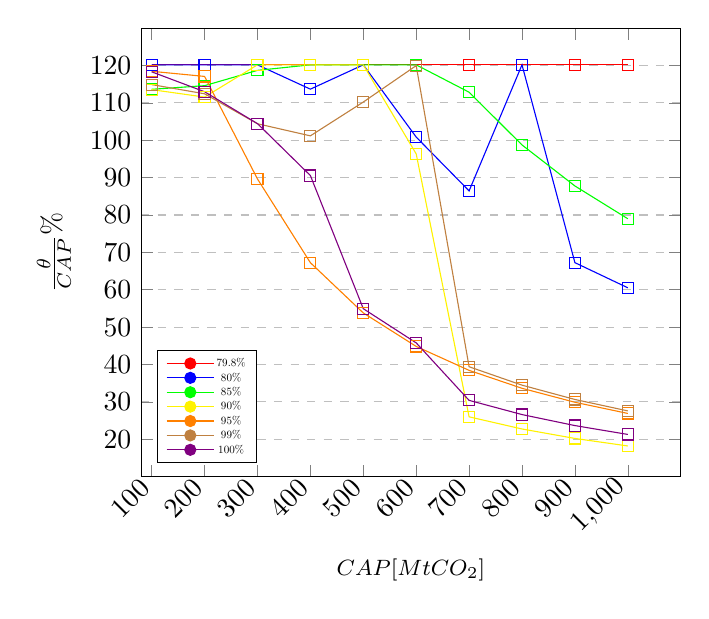
\begin{tikzpicture}
\centering
\begin{axis}[legend style={nodes={scale=0.4, transform shape}}, 
        legend image post style={mark=*},
    xlabel={{\footnotesize $CAP[MtCO_2]$}},
    ylabel={$\frac{\theta}{CAP}\%$},
    xmin=80, xmax=1100,
    ymin=10, ymax=130,
    xtick={100,200,300,400,500,600,700,800,900,1000},
    xticklabel style = {rotate=45,anchor=east},
    ytick={20,30,40,50,60,70,80,90,100,110,120},
    legend pos=south west,
    ymajorgrids=true,
    grid style=dashed,
]

\addplot[
    color=red,
    mark=square,
    ]
    coordinates {
    (100,120.2)(200,120.2)(300,120.2)(400,120.2)(500,120.2)(600,120.2)(700,120.2)(800,120.2)(900,120.2)(1000,120.2)
    };

\addplot[
    color=blue,
    mark=square,
    ]
    coordinates {
    (100,120.2)(200,120.2)(300,120.2)(400,113.69)(500,120.2)(600,100.87)(700,86.46)(800,120.2)(900,67.25)(1000,60.52)
    };
\addplot[
    color=green,
    mark=square,
    ]
    coordinates {
    (100,113.65)(200,114.62)(300,118.72)(400,120.2)(500,120.2)(600,120.2)(700,112.87)(800,98.76)(900,87.78)(1000,79)
    };
\addplot[
    color=yellow,
    mark=square,
    ]
    coordinates {
    (100,113.56)(200,111.57)(300,120.2)(400,120.2)(500,120.2)(600,96.37)(700,25.98)(800,22.73)(900,20.2)(1000,18.18)
    }; 
\addplot[
    color=orange,
    mark=square,
    ]
    coordinates {
    (100,118.47)(200,117.1)(300,89.66)(400,67.24)(500,53.79)(600,44.83)(700,38.42)(800,33.62)(900,29.88)(1000,26.89)
    };
\addplot[
    color=brown,
    mark=square,
    ]
    coordinates {
    (100,114.91)(200,112.45)(300,104.43)(400,101.19)(500,110.24)(600,119.99)(700,39.39)(800,34.46)(900,30.63)(1000,27.57)
    };
\addplot[
    color=violet,
    mark=square,
    ]
    coordinates {
    (100,118.33)(200,113)(300,104.46)(400,90.57)(500,54.93)(600,45.78)(700,30.39)(800,26.59)(900,23.64)(1000,21.27)
    };
    \legend{79.8\%, 80\%,85\%,90\%,95\%,99\%,100\%}  
\end{axis}

\end{tikzpicture}
}
\caption{{\footnotesize Ratio per CAP in Profit Oriented Model.}}
\label{rendcap}
\end{figure}

WHY IS THIS HAPPENING?? ANALISIS

To understand what is happening about the permit distribution between the different carbon emitters energy generators (carbon, gas and petro-diesel are considered), the model produces the results in Fig. \ref{petapaPO} and Fig. \ref{setapaPO}.

\begin{figure}[h]
  \centering
  \begin{minipage}[b]{0.49\textwidth}
    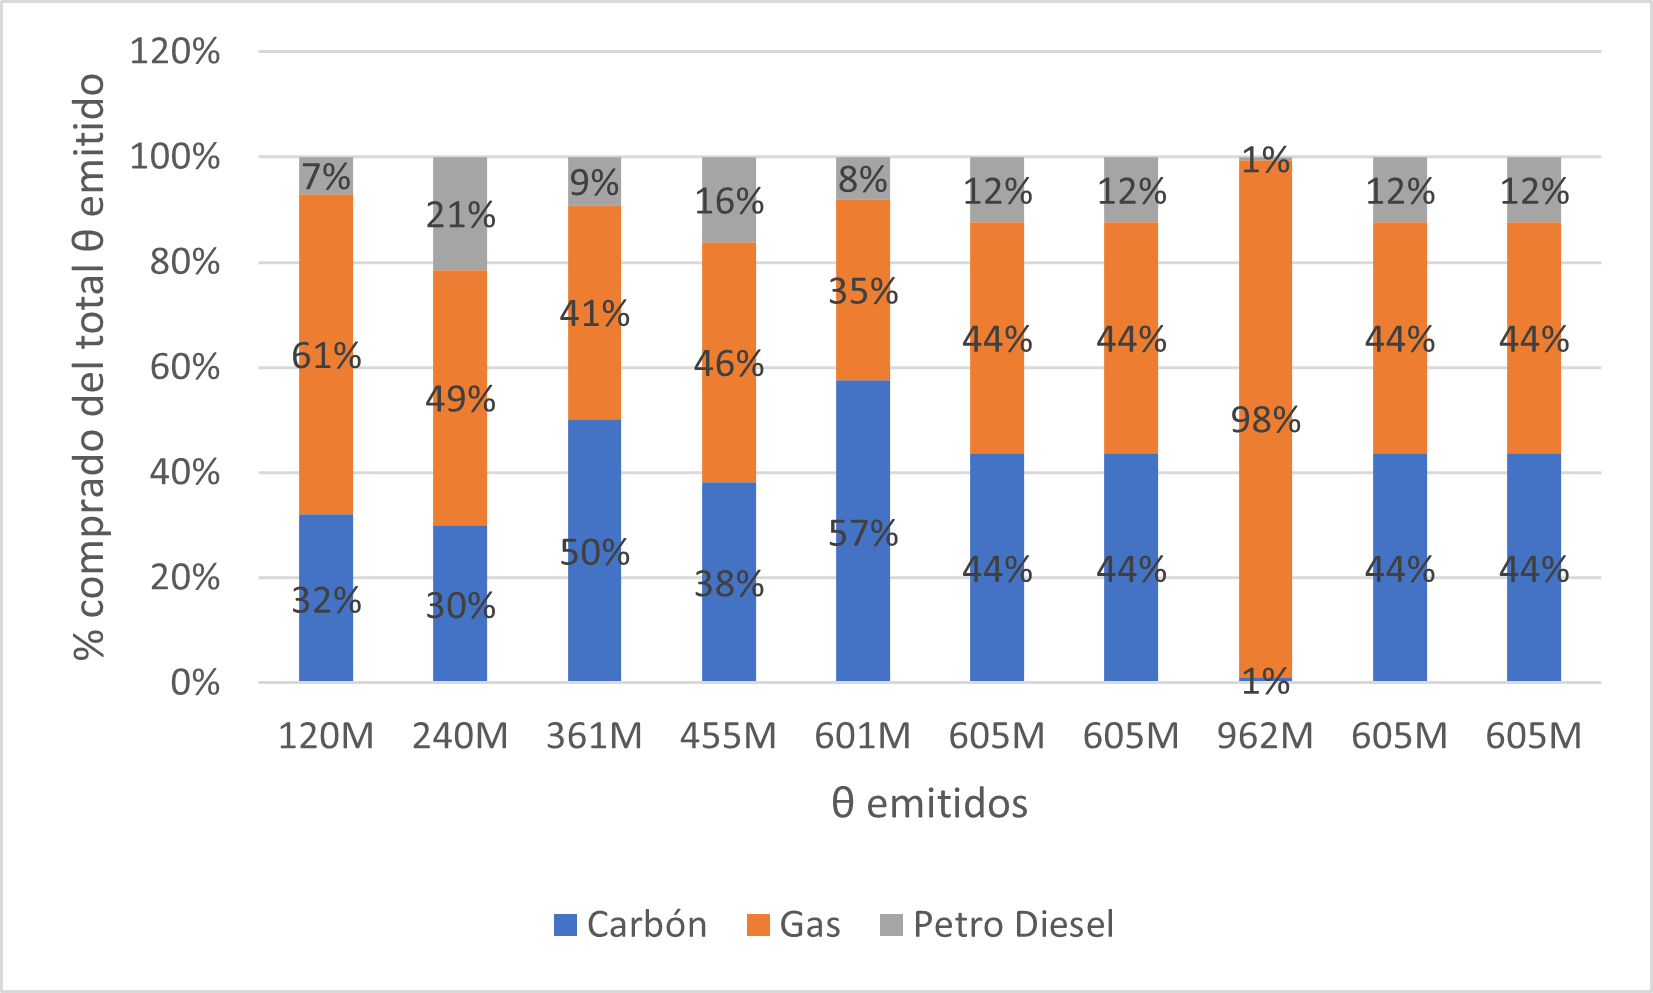
\includegraphics[width=\textwidth]{Submissions/EnergyPolicy/Images/distribucion primera etapa PO.png}
    \caption{{\footnotesize First stage and $P=80\%$.}}
    \label{petapaPO}
  \end{minipage}
  \hfill
  \begin{minipage}[b]{0.49\textwidth}
    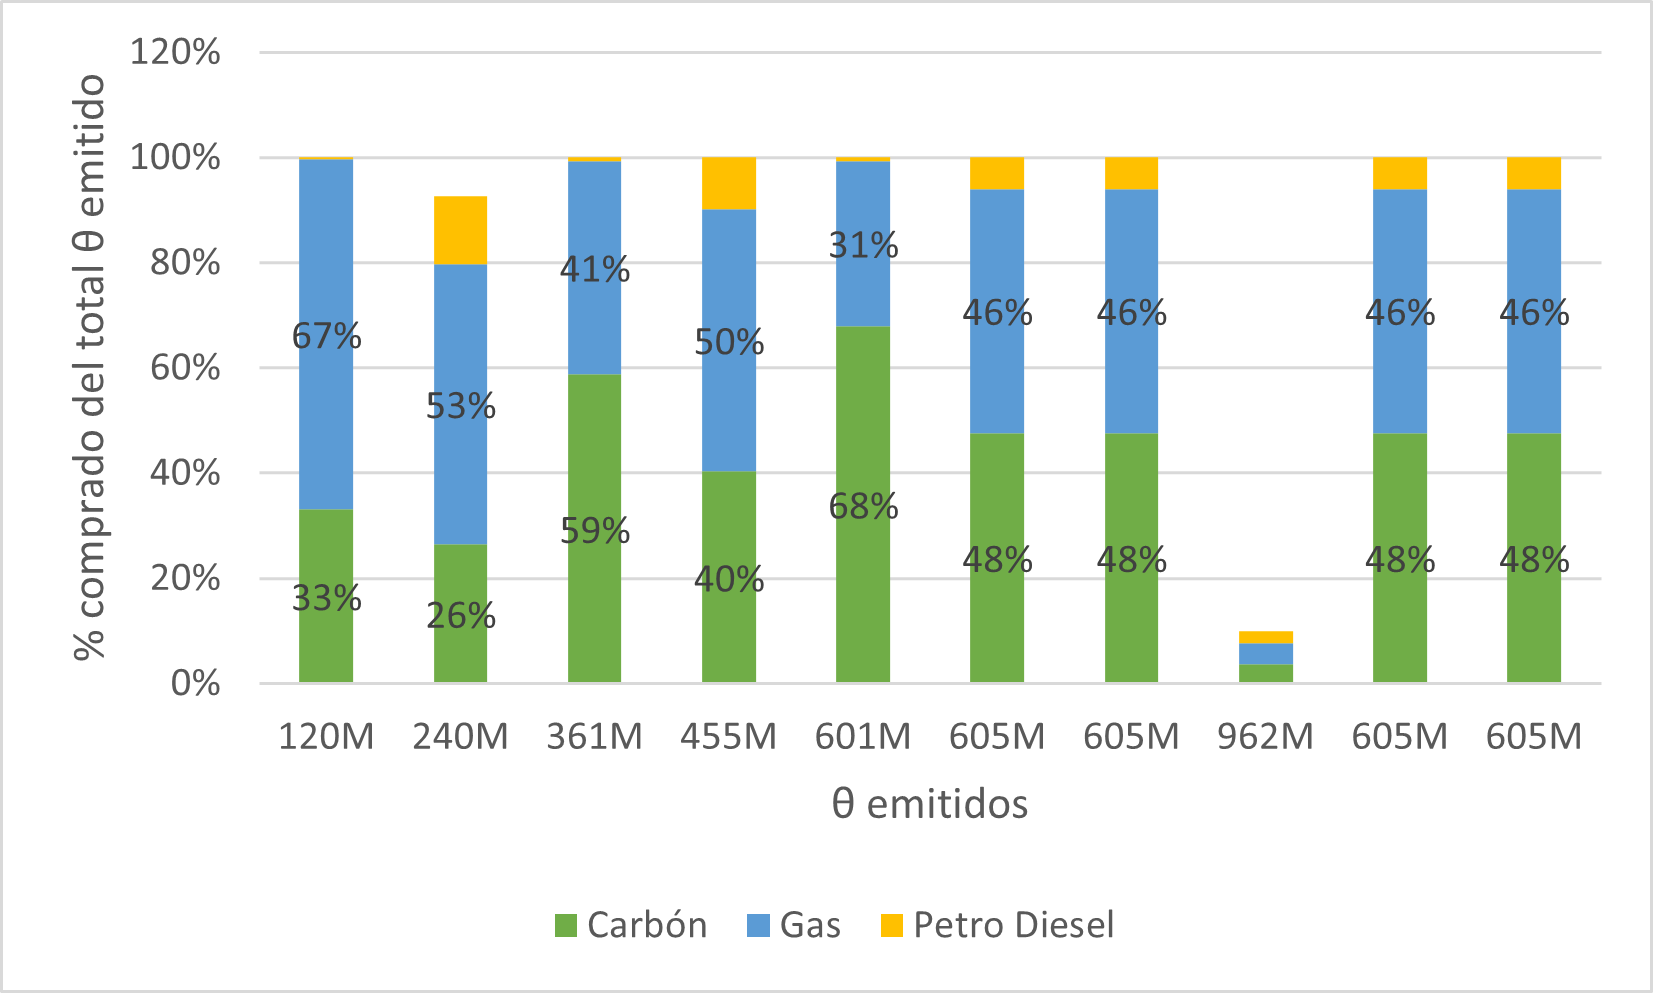
\includegraphics[width=\textwidth]{docs/DocumentoMemoria/core/images/distribucion segunda etapa.png}
    \caption{{\footnotesize Second stage and $P=80\%$.}}
    \label{setapaPO}
  \end{minipage}
\end{figure}

The first stage is when the Auctioneer decides the amount of permits to produce and sells them to the energy companies. Then, in the second stage, demand scenarios are revealed and a permit market is opened. This model in particular shows marginal change in the permit distribution for almost all carbon budgets. Coal base energy producers appear to have the most permits in both scenarios. There is an anomaly present when $CAP=800MtCO_2$ (962 million permits), it is possibly a solver error.

Other important variable to consider for the evaluation of this model is the electricity prices for the public per carbon budget. Table \ref{POpidporcap} shows interesting prices in the first stage, there appears to be an inverse effect on prices when the $\frac{\theta}{CAP}$ ratio increases.

\begin{table*}[t]
\caption{{\footnotesize Electricity prices ($\pi^d$) per CAP and $P=80\%$}}\label{POpidporcap}
\begin{footnotesize}
    \centering
    \begin{tabular}{ l l l l l l l l l l l }
    \hline
        $CAP$ & 100M & 200M & 300M & 400M & 500M & 600M & 700M & 800M & 900M & 1000M \\ \hline
        $\theta$  & 120M & 240M & 361M & 455M & 601M & 605M & 605M & 961M & 605M & 605M \\ \hline
        $\pi^d$  &  \$264.03   &  \$119.37   &  \$136.85   &  \$95.39   &  \$102.94   &  \$83.32   &  \$83.32   &  \$174.56   &  \$83.32   &  \$83.32   \\ \hline
    \end{tabular}
\end{footnotesize}
\end{table*}

Finally, the prices in the second stage can be evaluated for every demand scenario possible. The description of every demand scenario see \ref{Appendix:demandscenarios}. Fig. \ref{pidcap} shows that for the high GDP scenario (scenario 4) the prices are higher. On the other hand, there is an anomaly again in the $800MtCO_2$ budget.

\begin{figure}[h]
\centering
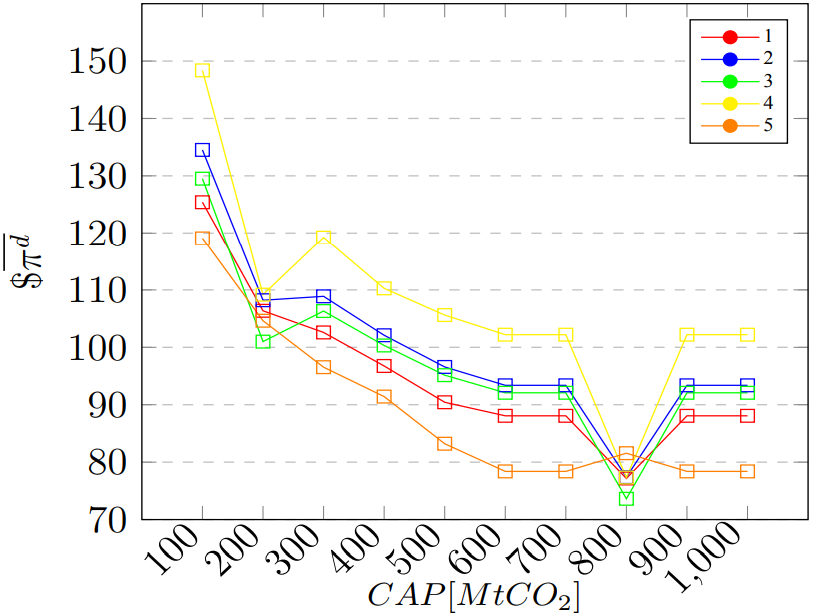
\includegraphics[width=8cm]{Submissions/EnergyPolicy/Images/Electricity prices per scenario PO.png}
\caption{{\footnotesize Average electricity prices(2019-2050) per demand scenario}}
\label{pidcap}
\end{figure}


\subsection{Quadratic Rate Welfare Oriented Model results}\label{subsec:resultsQR}

The Welfare Oriented version of the auctioneer model absolute value problem was solved in two different ways. The first one is modeled as follows:

\begin{equation}
\begin{array}{rrclcl}
\displaystyle \min_{\theta} & -\theta \pi^a + c(1-\frac{(\theta - \hat{\theta})^2}{\hat{\theta^2}}-d)^2 \\\textrm{s.a.} \label{fo:social1}\\
\end{array}
\end{equation}
\begin{equation}
\begin{array}{rrclcl}
\displaystyle \theta \pi^a - c(1-\frac{(\theta - \hat{\theta})^2}{\hat{\theta}^2}-d)^2 \geq 0 \qquad (\eta)\label{social1:r11}
\end{array}
\end{equation}
\begin{equation}
\begin{array}{rrclcl}
1 - \frac{(\theta-\hat{\theta})^2}{\hat{\theta}^2} - d \geq 0 \qquad (\mu) \label{social1:r31}
\end{array}
\end{equation}
\begin{equation}
\begin{array}{rrclcl}
\frac{(\theta-\hat{\theta})^2}{\hat{\theta}^2 }+ d \geq 0 \qquad (\lambda)\label{social1:r41}
\end{array}
\end{equation}
\begin{equation}
\begin{array}{rrclcl}
\theta \geq 0 \qquad (\varrho)\label{social1:r21}
\end{array}
\end{equation}

where the performance $P$ is now a variable formed as follows:

\begin{equation}
\begin{array}{rrclcl}
\displaystyle P = 1- (\frac{{\theta - \hat{\theta}}}{\hat{\theta}})^2 \\
\end{array}
\end{equation}

Like the previous model, this one is transformed into a MCP using the KKT conditions (see \ref{Appendix:mcpWOQR}) and solved using the PATH solver in GAMS. The first results are given by changing only the carbon budget in the interval $[100MtCO_2 , 1000MtCO_2]$. The resumed results of this exercise are showed in Table \ref{resultadostasacuadrada}.

\begin{table}[H]
    \centering
    \caption{{\footnotesize Quadratic Rate CAP variation results.}}
    \label{resultadostasacuadrada}
    \begin{tabular}{ l l l l l}
    \hline
        CAP & $\theta$ & Perf[P] & $\frac{\theta}{CAP}$  & $\pi^a$  \\ \hline
        100,000,000 & 144,944,410  & 0.798  & 1.449  &  \$232.82   \\ \hline
        200,000,000 & 289,888,820  & 0.798  & 1.449  &  \$141.56   \\ \hline
        300,000,000 & 434,833,230  & 0.798  & 1.449  &  \$103.33   \\ \hline
        400,000,000 & 579,777,640  & 0.798  & 1.449  &  \$-   \\ \hline
        500,000,000 & 653,754,577  & 0.905  & 1.308  &  \$37.27   \\ \hline
        600,000,000 & 619,939,821  & 0.999  & 1.033  &  \$40.43   \\ \hline
        700,000,000 & 661,258,561  & 0.997  & 0.945  &  \$36.42   \\ \hline
        800,000,000 & 610,913,181  & 0.944  & 0.764  &  \$31.28   \\ \hline
        900,000,000 & 609,127,279  & 0.896  & 0.677  &  \$31.21   \\ \hline
        1,000,000,000 & 698,676,376  & 0.909  & 0.699  &  \$30.00   \\ \hline
    \end{tabular}
\end{table}

The permits emitted by the Auctioneer seems to find a upper limit. The maximum permits created are $698,676,376$ even though the carbon budget is $1,000,000,000$ in that scenario. This shows that the attention concept inclusion enforces the model to produce around 600 million permits. In the bottom half of the budgets (100 to 400 million) emitting far from that enforced amount, appears to have a relation with low performances. On the other hand, the top 3 budgets (800, 900 and 1000 million) produce around 600 million permits, have a smaller $\frac{\theta}{CAP}$, have higher performances and the smallest permit prices. 

To understand the performance results through the carbon budgets, this relationship is graphed in Fig.\ref{rendcap}. This graph shows that there has to be a limit in the carbon budget between 400 and 500 million tons of $CO_2$ in which the performance changes and investment in information is elevated. Also there is a noticeable decrease in performance after the 700 million mark.

When compared with the results in Fig. \ref{rendcapTC2}, the decrease in ratio ($\frac{\theta}{CAP}$) coincides with the increase in performance showed in Fig.\ref{rendcap}. Like the last model, but in a lesser way, this model tends to decrease the amount of permits emitted the bigger the budget is. This is evidence of social benefit improvements because of the minimization of carbon pollution.   


\begin{figure}[h]
\centering
\resizebox{8cm}{6cm}{%
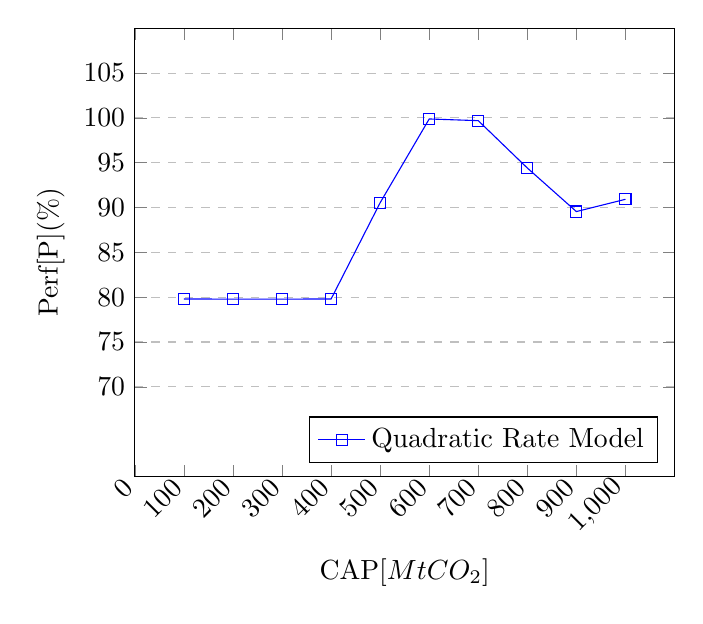
\begin{tikzpicture}
\begin{axis}[
    xlabel={CAP[$MtCO_2$]},
    ylabel={Perf[P](\%)},
    xmin=0, xmax=1100,
    ymin=60, ymax=110,
    xtick={0,100,200,300,400,500,600,700,800,900,1000},
    xticklabel style = {rotate=45,anchor=east},
    ytick={70,75,80,85,90,95,100,105},
    legend pos=south east,
    ymajorgrids=true,
    grid style=dashed,
]

\addplot[
    color=blue,
    mark=square,
    ]
    coordinates {
    (100,79.8)(200,79.79)(300,79.79)(400,79.8)(500,90.54)(600,99.88)(700,99.69)(800,94.41)(900,89.55)(1000,90.92)
    };
    \legend{Quadratic Rate Model}
    
\end{axis}
\end{tikzpicture}}
\caption{{\footnotesize Carbon budget effect on performance.}}
\label{rendcapTC}
\end{figure}

\begin{figure}[h]
\centering
\resizebox{8cm}{6cm}{%
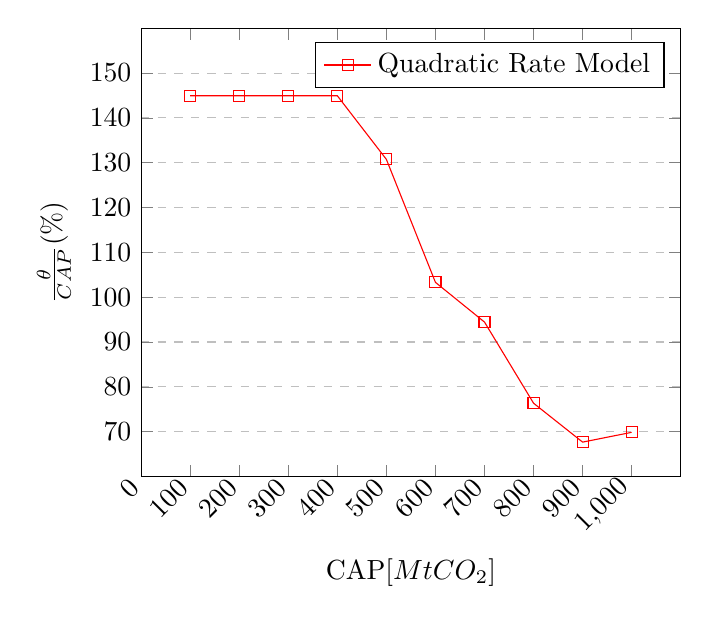
\begin{tikzpicture}
\begin{axis}[
    xlabel={CAP[$MtCO_2$]},
    ylabel={$\frac{\theta}{CAP}(\%)$},
    xmin=0, xmax=1100,
    ymin=60, ymax=160,
    xtick={0,100,200,300,400,500,600,700,800,900,1000},
    xticklabel style = {rotate=45,anchor=east},
    ytick={70,80,90,100,110,120,130,140,150},
    legend pos=north east,
    ymajorgrids=true,
    grid style=dashed,
]

\addplot[
    color=red,
    mark=square,
    ]
    coordinates {
    (100,144.94)(200,144.94)(300,144.94)(400,144.94)(500,130.75)(600,103.32)(700,94.46)(800,76.36)(900,67.68)(1000,69.86)
    };
    \legend{Quadratic Rate Model}
    
\end{axis}
\end{tikzpicture}}
\caption{{\footnotesize Carbon budget effect on ratio}}
\label{rendcapTC2}
\end{figure}

In regards to the permits distribution in this model in each scenario, like the previous model, coal base energy producers tends to be the dominant agent in the market. Fig. \ref{comptc1} and \ref{comptc2} graphs both scenarios of permit buying and distribution. 

\begin{figure}[h]
  \centering
  \begin{minipage}[b]{0.49\textwidth}
    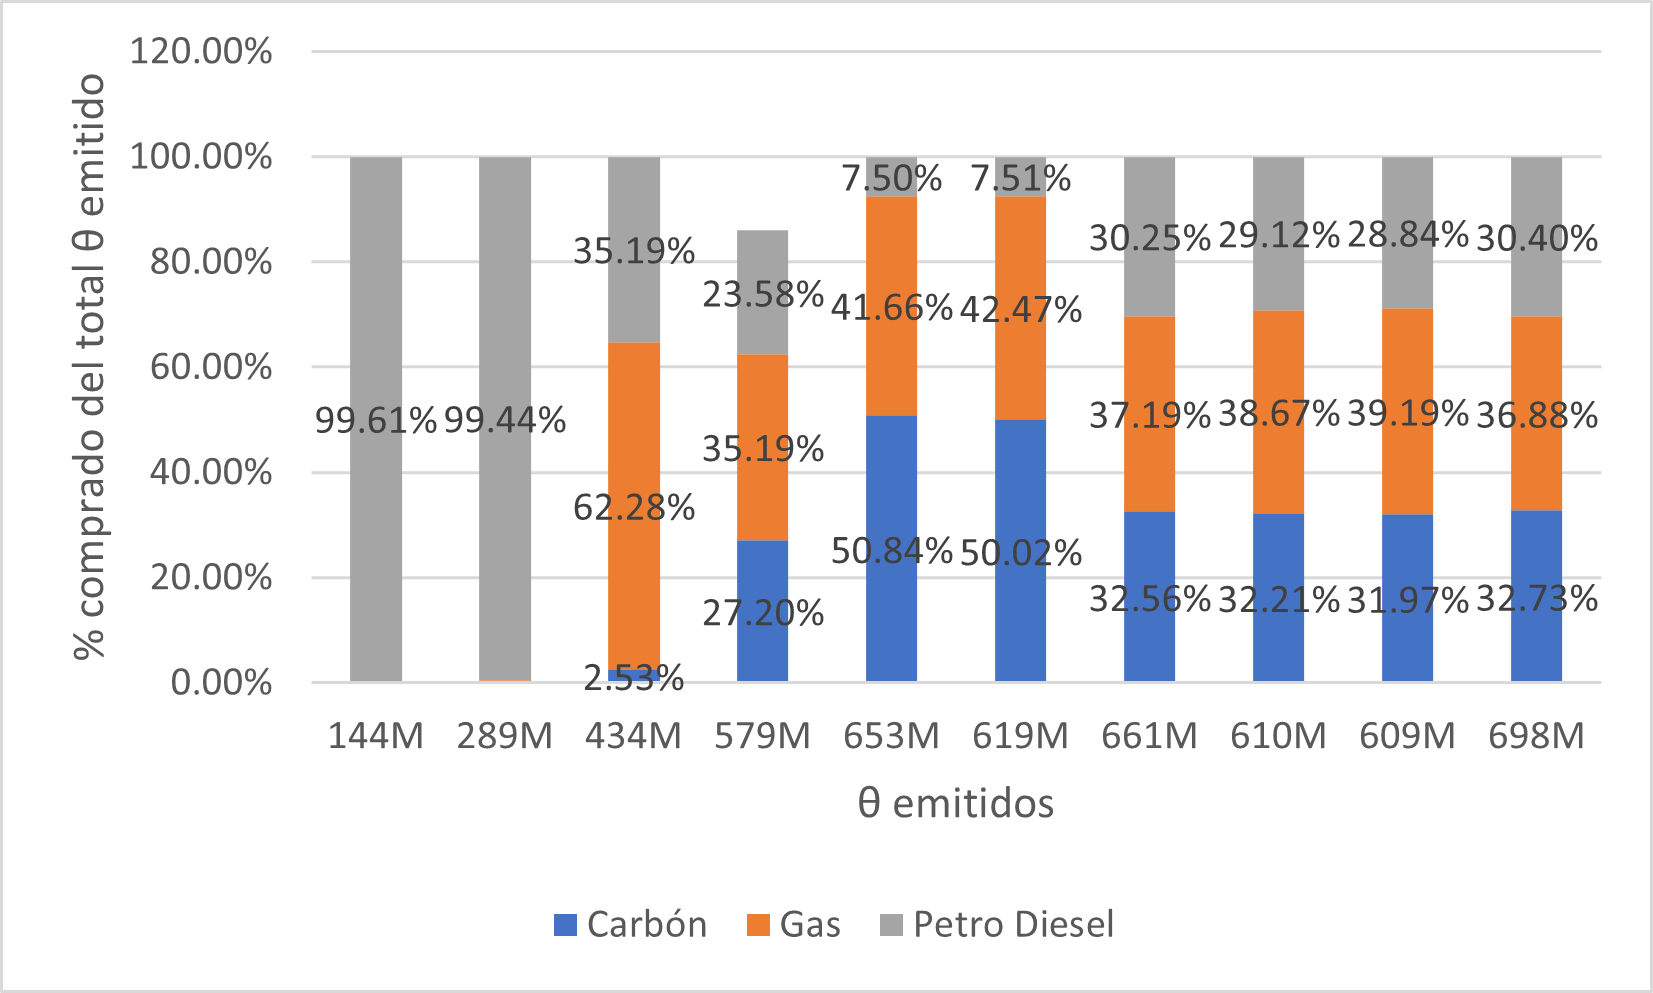
\includegraphics[width=\textwidth]{Submissions/EnergyPolicy/Images/distr primera etapa tasa cuadrada.png}
    \caption{{\footnotesize First stage distribution.}}
    \label{comptc1}
  \end{minipage}
  \hfill
  \begin{minipage}[b]{0.49\textwidth}
    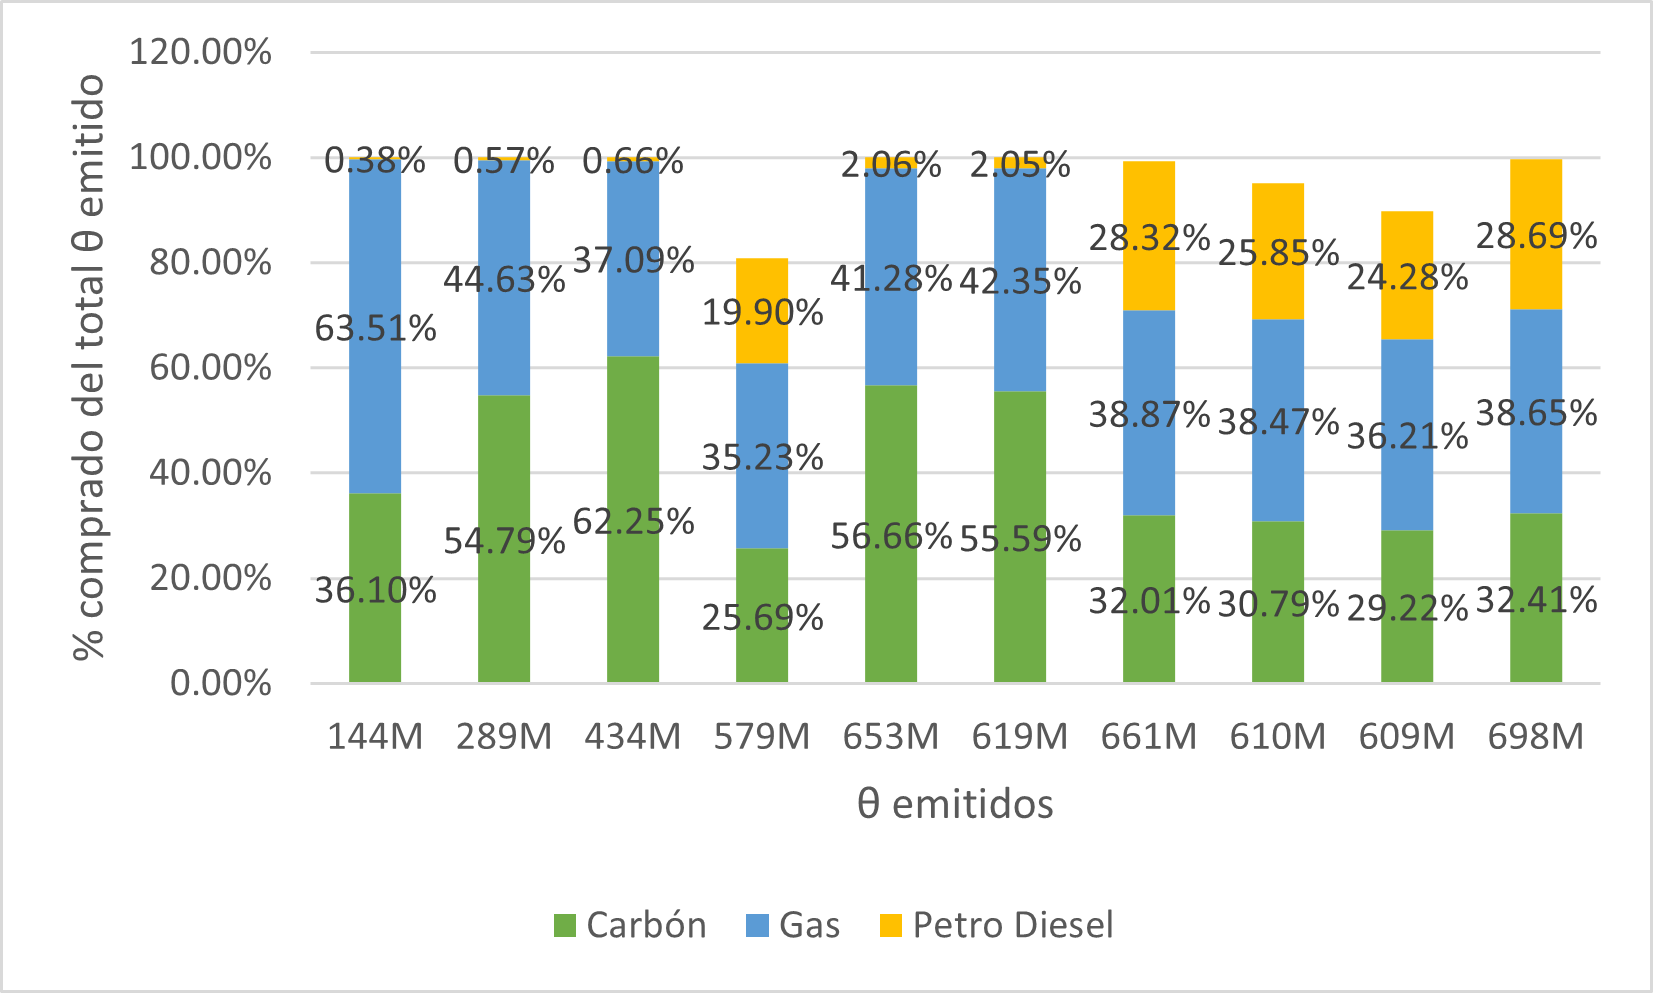
\includegraphics[width=\textwidth]{Submissions/EnergyPolicy/Images/distr segunda etapa tasa cuadrada.png}
    \caption{{\footnotesize Second stage distribution.}}
    \label{comptc2}
  \end{minipage}
\end{figure}

After the initial permits emission and energy generators buys, there is a equilibrium price found of the electricity for the public. Table \ref{TCpidporcap} shows similar prices for the top 6 carbon budgets (400 to 1000 $MtCO_2$), this may be related to the amount of permits emitted ($\theta$) in those budgets, where the Auctioneer sold around $600 MtCO_2$ in each one. 

\begin{table*}[b]
\caption{{\footnotesize Initial electricity prices ($\pi^d$) per CAP in Quadratic Rate Model.}}
    \label{TCpidporcap}
\begin{footnotesize}
    \centering
    \begin{tabular}{ l l l l l l l l l l l }
    \hline
        CAP[$MtCO_2$] & 100 & 200 & 300 & 400 & 500 & 600 & 700 & 800 & 900 & 1000 \\ \hline
       $\theta$[Millones]  & 145  & 290  & 435  & 580  & 654  & 620  & 661  & 611  & 609  & 699  \\ \hline
        $\pi^d$  &  \$232.54   &  \$155.49   &  \$123.21   &  \$93.90   &  \$87.48   &  \$90.44   &  \$105.74   &  \$95.05   &  \$93.38   &  \$94.53   \\ \hline
    \end{tabular}
\end{footnotesize}
\end{table*}

In the second stage, the demand scenarios are showed and the produces adapt their capacities. For each scenario and carbon budget, an average electricity was calculated to compare the scenarios in this model. Fig. \ref{TCrendcap} evidences similar differences between each scenario in comparison with the Profit Oriented Model. Nevertheless, this model spikes prices for all scenarios in the 700 million budget. This may be a indication that this particular model affects negatively social benefit by high electricity prices in some situations.

\begin{figure}[h]
\centering
\resizebox{8cm}{6cm}{%
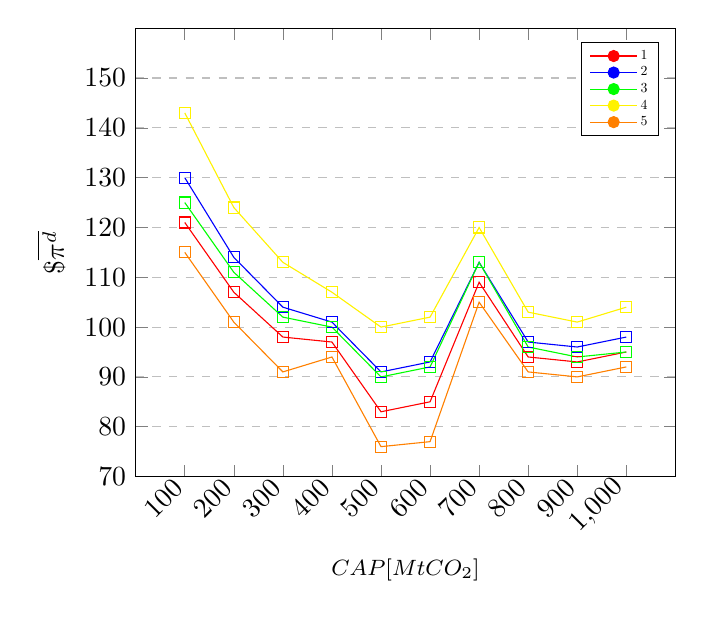
\begin{tikzpicture}
\centering
\begin{axis}[legend style={nodes={scale=0.5, transform shape}}, 
        legend image post style={mark=*},
    xlabel={{\footnotesize $CAP[MtCO_2]$}},
    xticklabel style = {rotate=45,anchor=east},
    ylabel={$\$ \overline{\pi^d}$},
    xmin=0, xmax=1100,
    ymin=70, ymax=160,
    xtick={100,200,300,400,500,600,700,800,900,1000},
    ytick={70,80,90,100,110,120,130,140,150},
    legend pos=north east,
    ymajorgrids=true,
    grid style=dashed,
]

\addplot[
    color=red,
    mark=square,
    ]
    coordinates {
    (100,121)(200,107)(300,98)(400,97)(500,83)(600,85)(700,109)(800,94)(900,93)(1000,95)
    };

\addplot[
    color=blue,
    mark=square,
    ]
    coordinates {(100,130)(200,114)(300,104)(400,101)(500,91)(600,93)(700,113)(800,97)(900,96)(1000,98)
    };
\addplot[
    color=green,
    mark=square,
    ]
    coordinates {
    (100,125)(200,111)(300,102)(400,100)(500,90)(600,92)(700,113)(800,96)(900,94)(1000,95)
    };
\addplot[
    color=yellow,
    mark=square,
    ]
    coordinates {
    (100,143)(200,124)(300,113)(400,107)(500,100)(600,102)(700,120)(800,103)(900,101)(1000,104)
    }; 
\addplot[
    color=orange,
    mark=square,
    ]
    coordinates {
   (100,115)(200,101)(300,91)(400,94)(500,76)(600,77)(700,105)(800,91)(900,90)(1000,92)
    };
    \legend{1,2,3,4,5}

\end{axis}
\end{tikzpicture}
}
\caption{{\footnotesize Average electricity prices (2019-2050)  per demand escenario Quadratic Rate Model.}}
\label{TCrendcap}
\end{figure}


\subsection{Precision Welfare Oriented Model results}\label{subsec:resultsPW}

The second version in which the absolute value problem is solved, is by transforming the numerator into a variable $r$.  The performance is now defined as $P= 1 - \frac{r}{\hat{\theta}}$. The complete model is as follows:


\begin{equation}
\begin{array}{rrclcl}
\displaystyle \min_{\theta,r} & -\theta \pi^a + c(1-\frac{r}{\hat{\theta}}-d)^2 \\\textrm{s.a.} \label{fo:social2}\\
\end{array}
\end{equation}
\begin{equation}
\begin{array}{rrclcl}
\displaystyle \theta \pi^a - c(1-\frac{r}{\hat{\theta}}-d)^2 \geq 0 \qquad (\eta)\label{social1:r12}
\end{array}
\end{equation}
\begin{equation}
\begin{array}{rrclcl}
\displaystyle r - \theta + \hat{\theta} \geq 0 \qquad (\lambda)\label{social1:r22}
\end{array}
\end{equation}
\begin{equation}
\begin{array}{rrclcl}
\displaystyle r + \theta - \hat{\theta} \geq 0 \qquad (\delta)\label{social1:r23}
\end{array}
\end{equation}
\begin{equation}
\begin{array}{rrclcl}
1-\frac{r}{\hat{\theta}}-d \geq 0 \qquad (\mu)\label{social1:r26}
\end{array}
\end{equation}
\begin{equation}
\begin{array}{rrclcl}
\frac{r}{\hat{\theta}} + d \geq 0 \qquad (\chi)\label{social1:r27}
\end{array}
\end{equation}
\begin{equation}
\begin{array}{rrclcl}
\theta \geq 0 \qquad (\varrho)\label{social1:r24}
\end{array}
\end{equation}
\begin{equation}
\begin{array}{rrclcl}
r \geq 0 \qquad (\alpha)\label{social1:r25}
\end{array}
\end{equation}

Equations \ref{social1:r22} and \ref{social1:r23} are included so the absolute value transformation is equivalent to this new definition. The main difference with the other modelations is the inclusion of a second variable. This one, as the others, is transformed into a MCP by the KKT conditions (see \ref{Appendix:mcpWOP}), coded into GAMS and solved with the PATH solver.

\begin{table}[h]
\caption{{\footnotesize Precision Model results.}}
    \label{resultadosprecision}
    \centering
    \begin{tabular}{ l l l l l }
    \hline
        CAP & $\theta$ & Perf[P] & $\frac{\theta}{CAP}$  & $\pi^a$ \\ \hline
        100,000,000 & 120,200,000  & 0.798  & 1.202  &  \$270.13   \\ \hline
        200,000,000 & 240,400,000  & 0.798  & 1.202  &  \$155.15   \\ \hline
        300,000,000 & 354,508,234  & 0.798  & 1.182  &  \$39.07   \\ \hline
        400,000,000 & 435,648,945  & 0.798  & 1.089  &  \$33.93   \\ \hline
        500,000,000 & 590,042,475  & 0.798  & 1.180  &  \$38.83   \\ \hline
        600,000,000 & 721,200,000  & 0.798  & 1.202  &  \$39.20   \\ \hline
        700,000,000 & 673,836,382  & 0.798  & 0.963  &  \$35.74   \\ \hline
        800,000,000 & 757,247,245  & 0.798  & 0.947  &  \$35.74   \\ \hline
        900,000,000 & 851,903,151  & 0.798  & 0.947  &  \$35.74   \\ \hline
        1,000,000,000 & 947,173,004  & 0.798  & 0.947  &  \$35.74   \\ \hline
    \end{tabular}
\end{table}


In this model, the results presented in Table \ref{resultadosprecision}, show that in this case the performance was unchanged for all the carbon budgets. With a constant value of 0.798, in a look that means that there was no investment in information to minimize the noise. Nevertheless, the $\frac{\theta}{CAP}$ ratio is different for almost every budget. Because of the way the performance was defined in the previous model, in that case there was a lineal relation between performance and the ratio. Also, there is at least intention of reducing the emitted permits, in most cases they are less than the limit 1.202 ratio, indicating that even though the model says that no additional information was bought, there is an intention to reduce carbon emissions.

The lack of clarity in this model shows there is space to improve it. There is conflicted analysis that can be related to bad formulation or lack of definition of the information acquisition.

\begin{figure}[h]
\centering
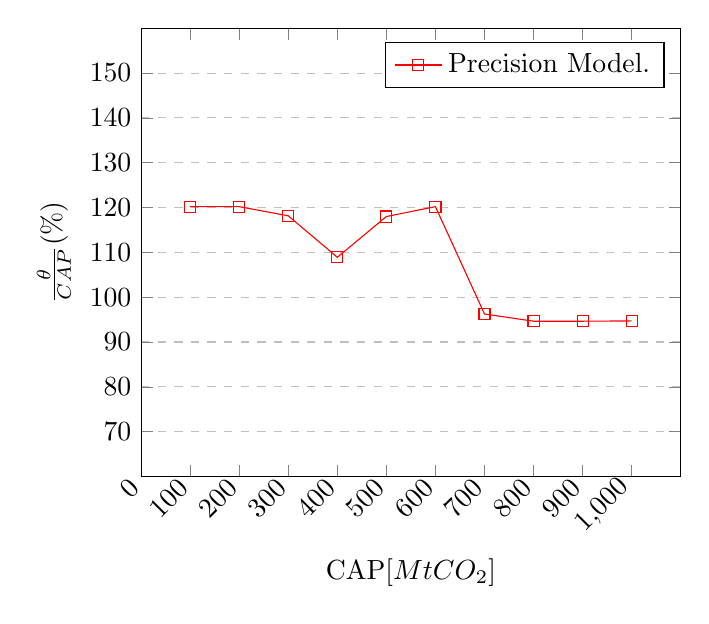
\begin{tikzpicture}
\begin{axis}[
    xlabel={CAP[$MtCO_2$]},
    ylabel={$\frac{\theta}{CAP}(\%)$},
    xmin=0, xmax=1100,
    ymin=60, ymax=160,
    xtick={0,100,200,300,400,500,600,700,800,900,1000},
    xticklabel style = {rotate=45,anchor=east},
    ytick={70,80,90,100,110,120,130,140,150},
    legend pos=north east,
    ymajorgrids=true,
    grid style=dashed,
]

\addplot[
    color=red,
    mark=square,
    ]
    coordinates {
    (100,120.2)(200,120.2)(300,118.16)(400,108.91)(500,118)(600,120.2)(700,96.26)(800,94.65)(900,94.65)(1000,94.71)
    };
    \legend{Precision Model.}
    
\end{axis}
\end{tikzpicture}
\caption{{\footnotesize CAP effect on ratio.}}
\label{rendcapMP2}
\end{figure}

Fig \ref{rendcapMP2} shows the ratios value for each carbon budget. The series has a apparent downtrend tendency. Again, this may be just a random result based on the high non lineal nature of the problem or, evidenced by the same tendency in the other two models, there is a direct effect on the auctioneer model to minimize pollution. Specially in larger budgets, because, the model understands there is a capacity to produce less permits.

The first and second stage permits distributions results in this model have some interesting contributions. One of the Chilean NDCs is to eliminate coal as energy fuel, so finding a model in which this product is efficiently eliminated would be of great aid. The results of this model in Fig. \ref{distriMP1} and Fig. \ref{distriMP3} show that coal ends up second in permit acquisition for all carbon budgets. This evidences a possibility for this model and the inclusion of rational attention in which direct and more specific objectives can be targeted and achieved.

Electricity prices in the first stage (shown in Table \ref{PMpidporcap}), present a low variance between CAP 300 and 1000. Complementing with the previous analysis made about the permits distribution, this prices may not variate a lot in the second stage and future prices because Fig. \ref{distriMP3} shows that for most of the carbon budgets there are less than 100\% of the permits in use. So, in this model, there is more electricity made by the renewable energy which in the short and medium term is more expensive.

Finally, Fig. \ref{PMrendcap} validates the last hypothesis. Showing that for all scenarios, there is no much variance in the prices. Having a mean close to a price of \$105 .

\begin{figure}[h]
  \centering
  \begin{minipage}[b]{0.49\textwidth}
    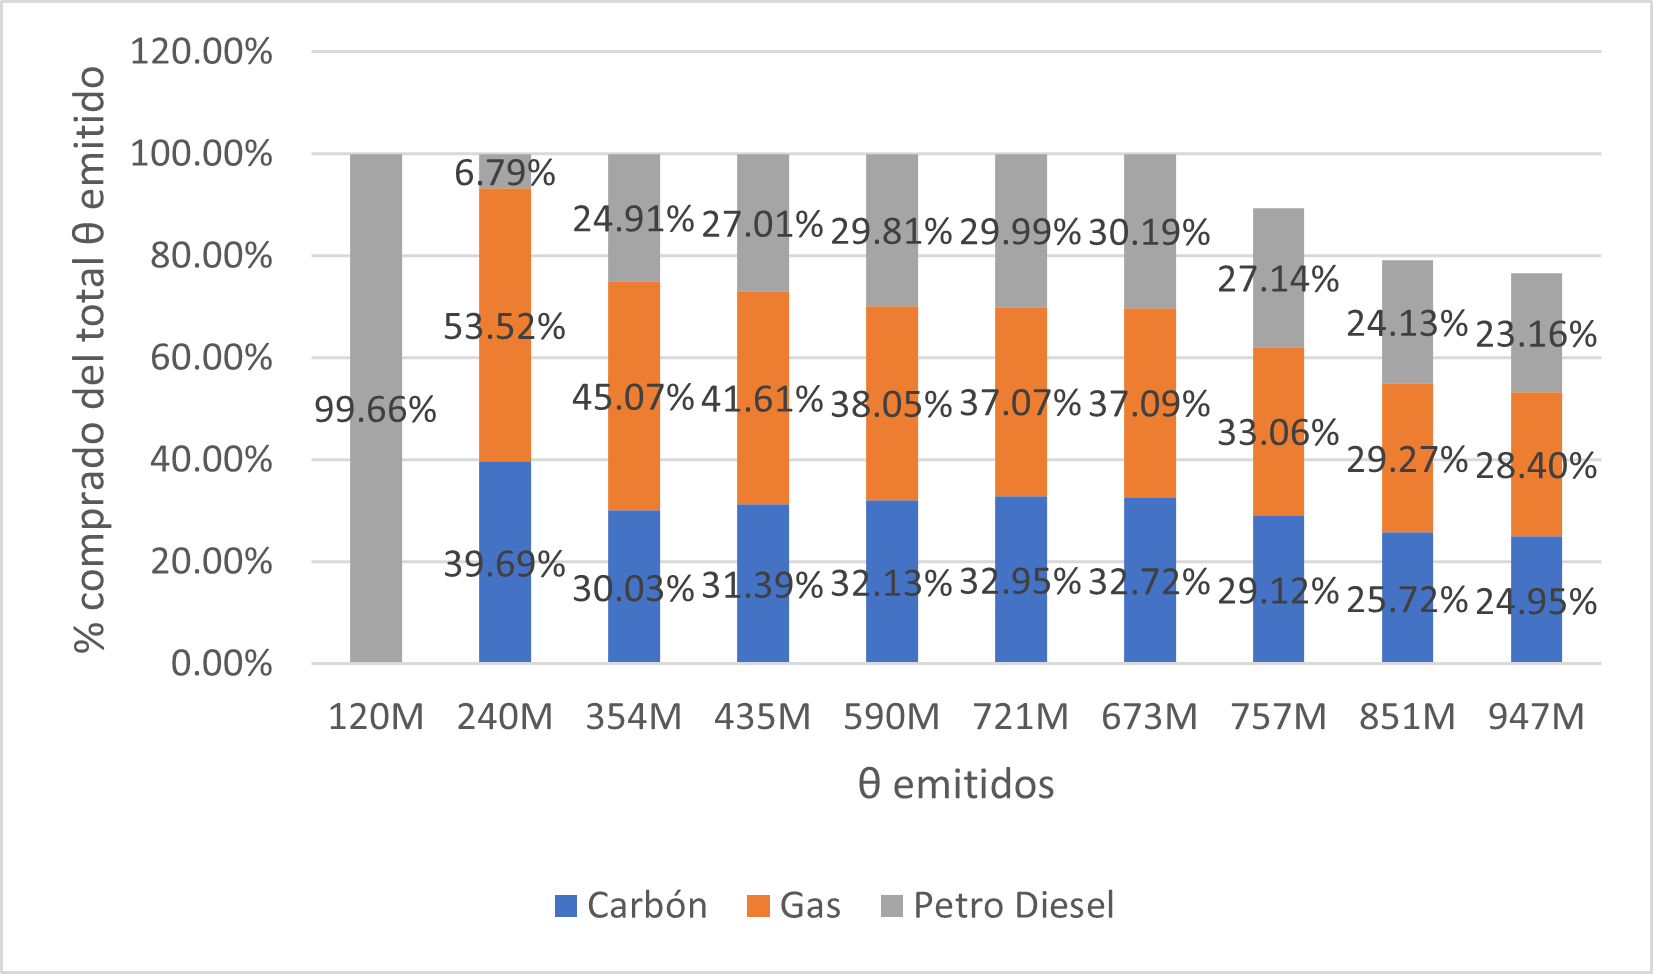
\includegraphics[width=\textwidth]{Submissions/EnergyPolicy/Images/distr primera etapa precision.png}
    \caption{{\footnotesize First Stage Distribution.}}
    \label{distriMP1}
  \end{minipage}
  \hfill
  \begin{minipage}[b]{0.49\textwidth}
    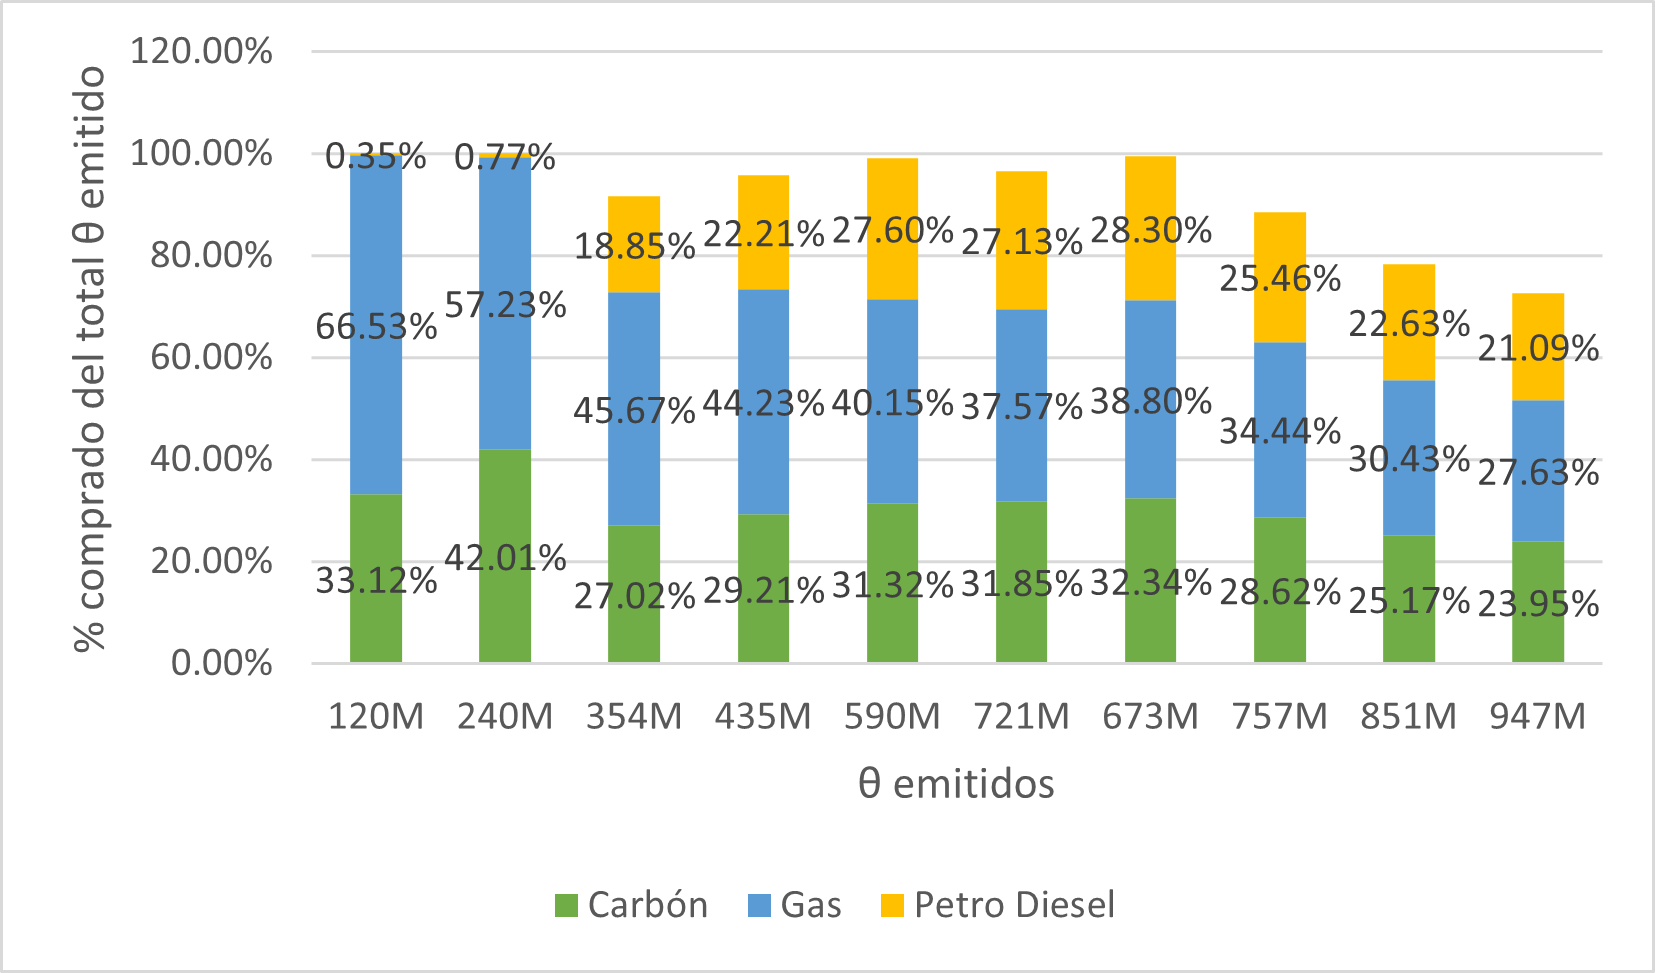
\includegraphics[width=\textwidth]{Submissions/EnergyPolicy/Images/distr segunda etapa precision.png}
    \caption{{\footnotesize Second Stage Distribution.}}
     \label{distriMP3}
  \end{minipage}
\end{figure}

\begin{table*}[b]
\caption{{\footnotesize Initial electricity prices ($\pi^d$) per CAP in Precision Model.}}
    \label{PMpidporcap}
\begin{footnotesize}
    \centering
    \begin{tabular}{ l l l l l l l l l l l }
    \hline
        CAP[$MtCO_2$] & 100 & 200 & 300 & 400 & 500 & 600 & 700 & 800 & 900 & 1000 \\ \hline
          $\theta$[Millones] & 120 & 240 & 355 & 436 & 590 & 721 & 674 & 757 & 852 & 947 \\ \hline
    $\pi^d$  &  \$264.03   &  \$169.98   &  \$106.88   &  \$98.92   &  \$110.36   &  \$93.00   &  \$105.33   &  \$99.07   &  \$97.95   &  \$92.09   \\ \hline
    \end{tabular}
\end{footnotesize}
\end{table*}

\begin{figure}[h]
\centering
\resizebox{8cm}{6cm}{%
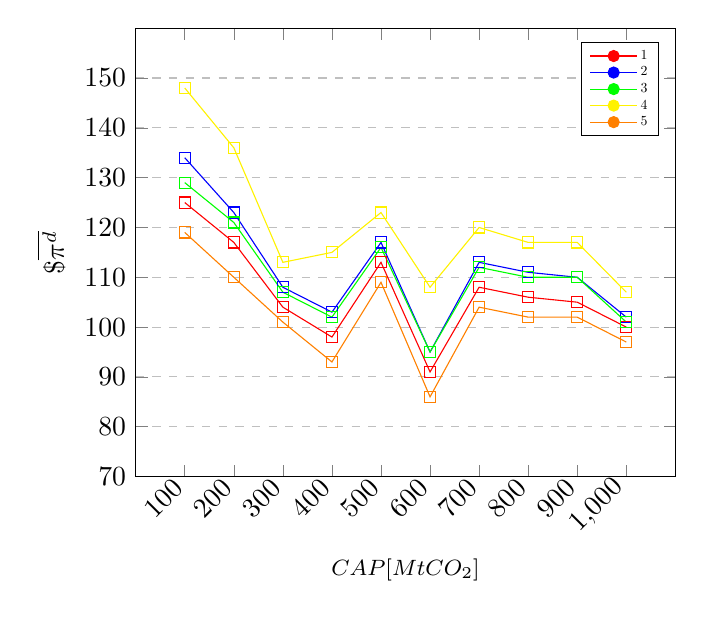
\begin{tikzpicture}
\centering
\begin{axis}[legend style={nodes={scale=0.5, transform shape}}, 
        legend image post style={mark=*},
    xlabel={{\footnotesize $CAP[MtCO_2]$}},
    xticklabel style = {rotate=45,anchor=east},
    ylabel={$\$ \overline{\pi^d}$},
    xmin=0, xmax=1100,
    ymin=70, ymax=160,
    xtick={100,200,300,400,500,600,700,800,900,1000},
    ytick={70,80,90,100,110,120,130,140,150},
    legend pos=north east,
    ymajorgrids=true,
    grid style=dashed,
]

\addplot[
    color=red,
    mark=square,
    ]
    coordinates {
    (100,125)(200,117)(300,104)(400,98)(500,113)(600,91)(700,108)(800,106)(900,105)(1000,100)
    };

\addplot[
    color=blue,
    mark=square,
    ]
    coordinates {(100,134)(200,123)(300,108)(400,103)(500,117)(600,95)(700,113)(800,111)(900,110)(1000,102)
    };
\addplot[
    color=green,
    mark=square,
    ]
    coordinates {
    (100,129)(200,121)(300,107)(400,102)(500,116)(600,95)(700,112)(800,110)(900,110)(1000,101)
    };
\addplot[
    color=yellow,
    mark=square,
    ]
    coordinates {
    (100,148)(200,136)(300,113)(400,115)(500,123)(600,108)(700,120)(800,117)(900,117)(1000,107)
    }; 
\addplot[
    color=orange,
    mark=square,
    ]
    coordinates {
    (100,119)(200,110)(300,101)(400,93)(500,109)(600,86)(700,104)(800,102)(900,102)(1000,97)
    };

    \legend{1,2,3,4,5}

\end{axis}
\end{tikzpicture}
}
\caption{{\footnotesize Electricity prices (2019-2050) per scenario}}
\label{PMrendcap}
\end{figure}



\newpage
\subsection{Models comparison}\label{subsec:resultscomparison}

For this final part, we make a comparison between the 3 models presented in this work and the results of the original model proposed by \cite{amigo_two_2021}. The idea of this is to understand the impact of including the rational inattention concept into the model by comparing the models profits, social benefits and main results about prices and permits. This comparison can result in conclusions about what is the best model or more suitable for the Chilean NDC and other countries NDCs.

The work made in this paper is a first inclusion of the rational inattention concept introduced in a model of this type, maybe the first made in the electric industry. Because of this, this models are not to be used in real applications but are made for research only. We established as the main objective to identify if the inclusion of rational inattention does enhance social benefit by resulting in lower prices, lower permits emitted and lower carbon emissions. To quantify this, we established as a objective that one the the versions of the models presented in this work has to have less permits and lower prices in 40\% of the cases.


In Fig. \ref{utilidades}, the results show that the original model produce higher profits for the auctioneer in 70\% of the carbon budgets. On the one hand, it is important to mention that no expenses were considered for the auctioneer in this model since its objective function only considered a cost called the Social Cost of Carbon. The former was ignored in the equilibrium model solution since it was considered independent of the permissions issued ($\theta$) by the original authors.

On the other hand, the reformulated models take the value of the costs of additional information $c$ by calibrating them with the original. Therefore, taking into account the auctioneer's profits for these models is also not the most important indicator to consider. Additionally, considering profits as an indicator for success in a public program is generally not the main objective, its overhead ratio may be a better one. In a later work, it is expected to calculate these costs in a real way and consider the operational costs for a real time implementation of the model.

Permit sales prices are an indicator of the quantity of permits issued since these obey the law of demand. They are also an indicator of the costs associated with the permit production. Fig. \ref{piapormodelo} shows that the original model has the largest prices for all carbon budgets. This may be an indicator that the new models are looking for
with a greater effect on social welfare, since, despite the fact that these have production costs, they do not transfer these costs to the permits, potentially producing, lower electricity costs.

On the contrary, these prices may be the product of more permits issued, and therefore, more emissions into the environment, producing more carbon and affecting social wellness. 


\begin{figure}[h]
    \centering
    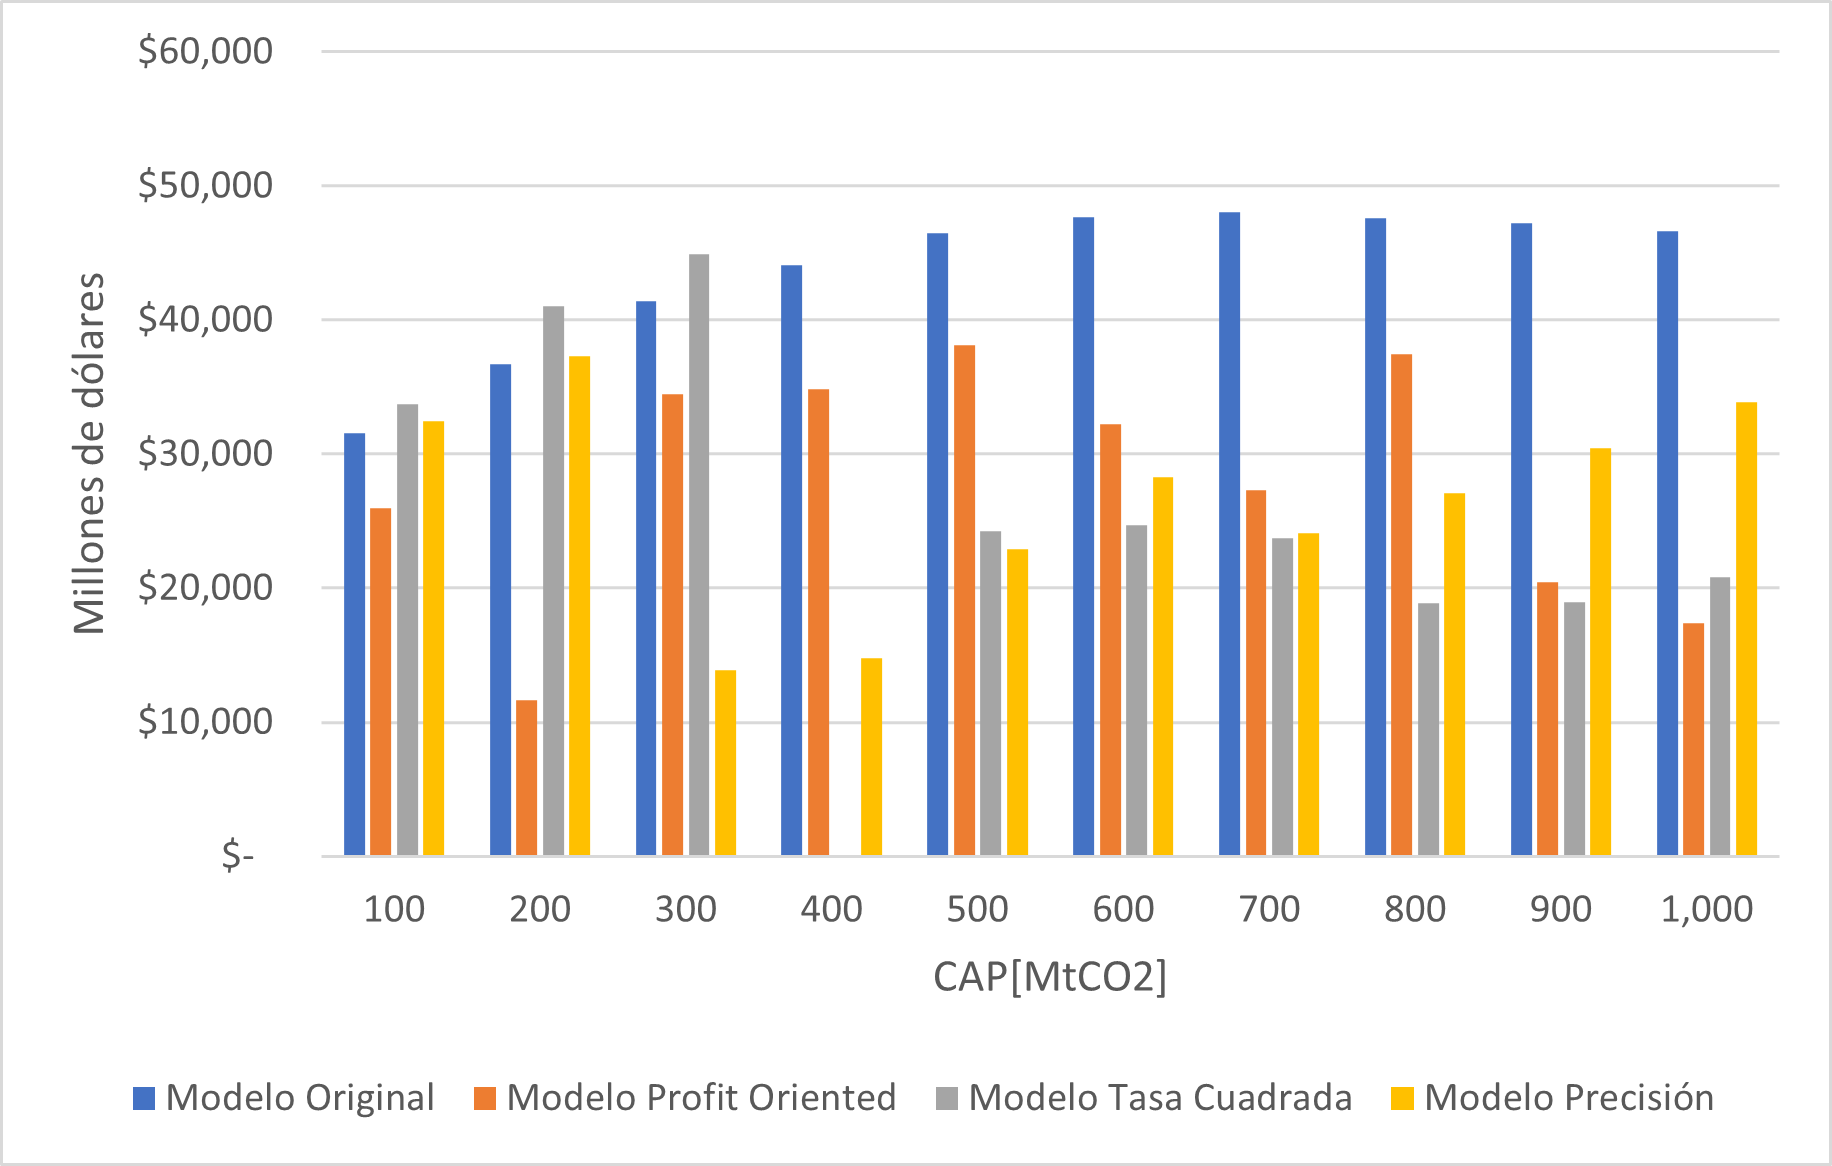
\includegraphics[width=8cm]{Submissions/EnergyPolicy/Images/utilidad de todos lo modelos.png}
\caption{{\footnotesize Auctioneer profit per model.}}
    \label{utilidades}
\end{figure}

\begin{figure}[h]
\centering
\resizebox{8cm}{6cm}{%
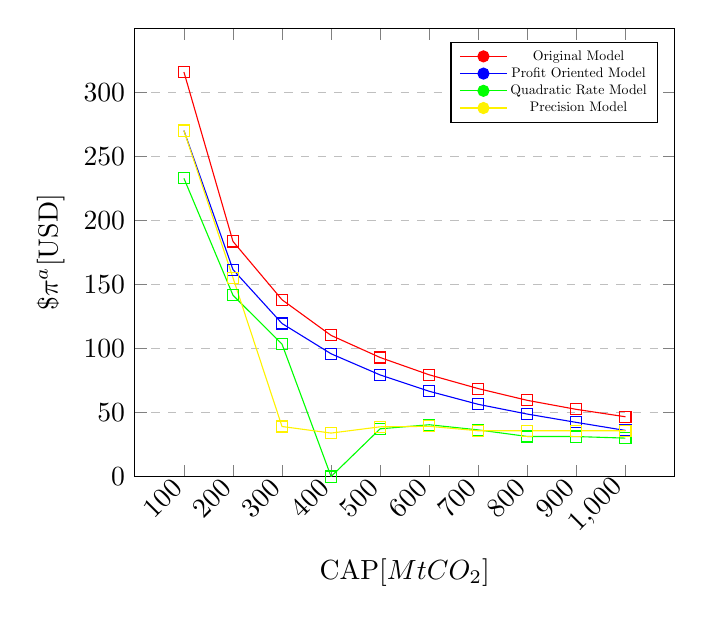
\begin{tikzpicture}
\centering
\begin{axis}[legend style={nodes={scale=0.5, transform shape}}, 
        legend image post style={mark=*},
    xlabel={CAP[$MtCO_2$]},
    ylabel={$\$ \pi^a$[USD]},
    xmin=0, xmax=1100,
    ymin=0, ymax=350,
    xtick={100,200,300,400,500,600,700,800,900,1000},
    xticklabel style = {rotate=45,anchor=east},
     ytick={0,50,100,150,200,250,300},
    legend pos=north east,
    ymajorgrids=true,
    grid style=dashed,
]

\addplot[
    color=red,
    mark=square,
    ]
    coordinates {
    (100,315.82)(200,183.55)(300,138.01)(400,110.18)(500,92.93)(600,79.42)(700,68.65)(800,59.48)(900,52.43)(1000,46.66)
    };

\addplot[
    color=blue,
    mark=square,
    ]
    coordinates {(100,270.12)(200,161.56)(300,119.47)(400,95.83)(500,79.31)(600,66.57)(700,56.37)(800,48.76)(900,42.26)(1000,35.98)

    };
    
\addplot[
    color=green,
    mark=square,
    ]
    coordinates {
    (100,232.82)(200,141.55)(300,103.32)(400,0)(500,37.26)(600,40.43)(700,36.41)(800,31.27)(900,31.21)(1000,30)

    };
    
\addplot[
    color=yellow,
    mark=square,
    ]
    coordinates {
    (100,270.12)(200,155.15)(300,39.06)(400,33.93)(500,38.82)(600,39.2)(700,35.73)(800,35.73)(900,35.73)(1000,35.73)


    }; 
    \legend{Original Model, Profit Oriented Model,Quadratic Rate Model,Precision Model}

\end{axis}
\end{tikzpicture}
}
\caption{{\footnotesize Permit prices $\pi^a$ per CAP}}
\label{piapormodelo}
\end{figure}

On the contrary, these prices may be the product of more permits issued, and therefore, more emissions into the environment, producing more carbon and affecting social wellness.

\begin{figure}[h]
\centering
\resizebox{8cm}{6cm}{%
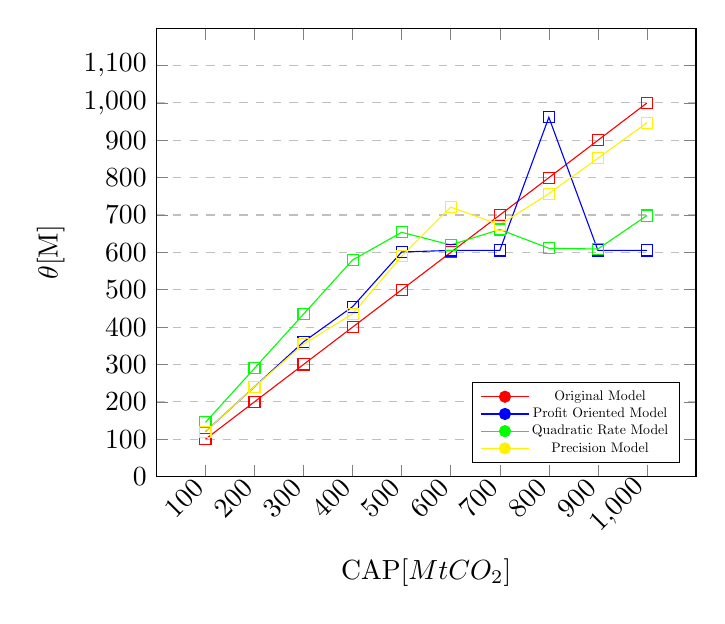
\begin{tikzpicture}
\centering
\begin{axis}[legend style={nodes={scale=0.5, transform shape}}, 
        legend image post style={mark=*},
    xlabel={CAP[$MtCO_2$]},
    ylabel={$\theta$[M]},
    xmin=0, xmax=1100,
    ymin=0, ymax=1200,
    xtick={100,200,300,400,500,600,700,800,900,1000},
    xticklabel style = {rotate=45,anchor=east},
    ytick={0,100,200,300,400,500,600,700,800,900,1000,1100},
    legend pos=south east,
    ymajorgrids=true,
    grid style=dashed,
]

\addplot[
    color=red,
    mark=square,
    ]
    coordinates {
    (100,100)(200,200)(300,300)(400,400)(500,500)(600,600)(700,700)(800,800)(900,900)(1000,1000)
    };

\addplot[
    color=blue,
    mark=square,
    ]
    coordinates {(100,120.2)(200,240.4)(300,360.6)(400,454.79)(500,601)(600,605.27)(700,605.27)(800,961.6)(900,605.27)(1000,605.27)
    };
    
\addplot[
    color=green,
    mark=square,
    ]
    coordinates {
    (100,144.94)(200,289.88)(300,434.83)(400,579.77)(500,653.75)(600,619.93)(700,661.25)(800,610.91)(900,609.12)(1000,698.67)
    };
    
\addplot[
    color=yellow,
    mark=square,
    ]
    coordinates {
    (100,120.2)(200,240.4)(300,354.5)(400,435.64)(500,590.04)(600,721.2)(700,673.83)(800,757.24)(900,851.9)(1000,947.17)
    }; 
    \legend{Original Model, Profit Oriented Model,Quadratic Rate Model,Precision Model}

\end{axis}
\end{tikzpicture}
}
\caption{{\footnotesize Permits emitted per CAP}}
\label{permisospormodelo}
\end{figure}

Figure \ref{permisospormodelo} shows that the previous analysis is not true for all cases. In the first 5 established CAPs, the auctioneer in the original model issues fewer permits than the new versions, but, in $CAP=600$ the Square Rate model issues a very similar amount of permits and in the following ones, it issues fewer permits, resulting in lower emissions. Also, the other two models (Precision and Profit Oriented) issue fewer permits in 3 and 4 of the last 5 CAPs, respectively.

Thanks to the previous statement, the criteria mentioned at the beginning of this subchapter is met to validate the use of rational care in this system, since one of the models has fewer permits issued in more than $40\%$ of the CAPs, but the Most notable is that all models have 3 or more CAPs with lower emissions than the original model.

Finally, electricity prices for individuals are compared between the models in each carbon budget. Figure \ref{pidpormodelo} demonstrates that the Profit Oriented and Quadratic Rate models create lower prices for individuals in $60\%$ of the CAPs. In particular, the Profit Oriented does it for $80\%$ of them. 

It is important to note that this last statement is true, partially, because of higher permits emitted than the original model so non green companies create more electricity (its cheaper), in many carbon budgets this is not the case. This brings into perspective that the inclusion of rational inattention does decrease energy prices and impacts positively in social well being. 

It is important now to evaluate why is this happening, why does the model create cheaper electricity prices but at the same time reduces carbon? 

\begin{figure}[h]
\centering
\resizebox{8cm}{6cm}{%
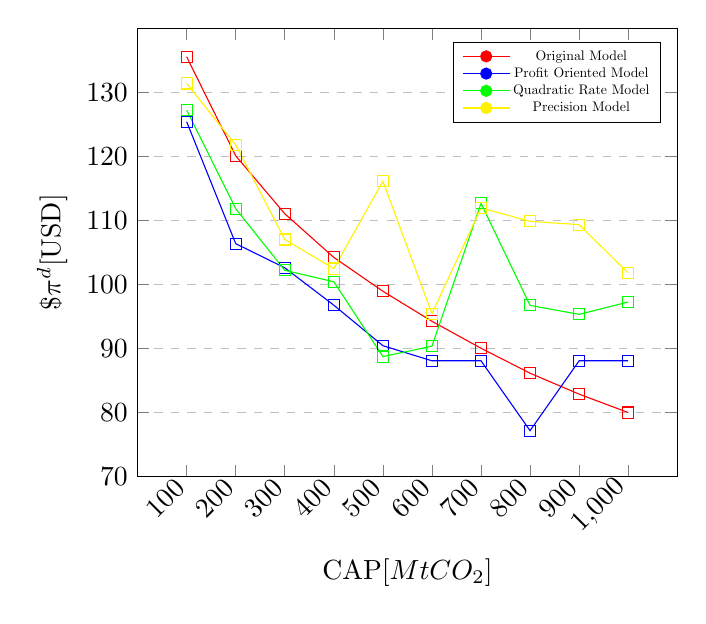
\begin{tikzpicture}
\centering
\begin{axis}[legend style={nodes={scale=0.5, transform shape}}, 
        legend image post style={mark=*},
    xlabel={CAP[$MtCO_2$]},
    ylabel={$\$ \pi^d$[USD]},
    xmin=0, xmax=1100,
    ymin=70, ymax=140,
    xtick={100,200,300,400,500,600,700,800,900,1000},
    xticklabel style = {rotate=45,anchor=east},
     ytick={70,80,90,100,110,120,130},
    legend pos=north east,
    ymajorgrids=true,
    grid style=dashed,
]

\addplot[
    color=red,
    mark=square,
    ]
    coordinates {
    (100,135.54)(200,120.08)(300,111.03)(400,104.21)(500,98.93)(600,94.24)(700,90.03)(800,86.13)(900,82.86)(1000,79.99)

    };

\addplot[
    color=blue,
    mark=square,
    ]
    coordinates {
    (100,125.4)(200,106.36)(300,102.59)(400,96.75)(500,90.43)(600,88.07)(700,88.07)(800,77.16)(900,88.07)(1000,88.07)

    };
    
\addplot[
    color=green,
    mark=square,
    ]
    coordinates {
    (100,127.22)(200,111.82)(300,102.2)(400,100.41)(500,88.73)(600,90.35)(700,112.66)(800,96.72)(900,95.32)(1000,97.25)
    };
    
\addplot[
    color=yellow,
    mark=square,
    ]
    coordinates {
    (100,131.38)(200,121.78)(300,107.01)(400,102.47)(500,116.1)(600,95.43)(700,111.93)(800,109.85)(900,109.33)(1000,101.77)
    }; 
    \legend{Original Model, Profit Oriented Model,Quadratic Rate Model,Precision Model}

\end{axis}
\end{tikzpicture}
}
\caption{{\footnotesize Electricity average price (2019-2050) $\pi^d$ per CAP.}}
\label{pidpormodelo}
\end{figure}


\newpage
\section{Conclusion}



% Numbered list
% Use the style of numbering in square brackets.
% If nothing is used, default style will be taken.
%\begin{enumerate}[a)]
%\item 
%\item 
%\item 
%\end{enumerate}  

% Unnumbered list
%\begin{itemize}
%\item 
%\item 
%\item 
%\end{itemize}  

% Description list
%\begin{description}
%\item[]
%\item[] 
%\item[] 
%\end{description}  

% Figure
%\begin{figure}[<options>]
%	\centering
%		\includegraphics[<options>]{}
%	  \caption{}\label{fig1}
%\end{figure}


%\begin{table}[<options>]
%\caption{}\label{tbl1}
%\begin{tabular*}{\tblwidth}{@{}LL@{}}
%\toprule
%  &  \\ % Table header row
%\midrule
% & \\
% & \\
% & \\
% & \\
%\bottomrule
%\end{tabular*}
%\end{table}

% Uncomment and use as the case may be
%\begin{theorem} 
%\end{theorem}

% Uncomment and use as the case may be
%\begin{lemma} 
%\end{lemma}

%% The Appendices part is started with the command \appendix;
%% appendix sections are then done as normal sections
\newpage
\appendix
\section{Appendix A}

\subsection{MCP Auctioneer Profit Oriented}\label{AMCPPO}

\begin{align}
0\leq -P\pi^a(1+\eta) + \mu \perp \theta \geq 0 \label{compllag33}\\
0 \leq \theta \pi^a P - c(P-d)^2 \perp \eta \geq 0 \label{compllag331}\\
0 \leq \hat{\theta}(1+ error) - \theta \perp \mu \geq 0 \label{compllag332}
\end{align}

\subsection{MCP Auctioneer Welfare Oriented Quadratic Rate}\label{Appendix:mcpWOQR}


\begin{table*}
\begin{footnotesize}
\begin{align}
0 \leq \theta \perp - \pi^a + c(-2\theta + 2\hat{\theta})\frac{(2-2d-2(\frac{\theta - \hat{\theta}}{\hat{\theta}})^2)}{\hat{\theta}^2} - \eta \pi^a + c\eta((-2\theta + 2\hat{\theta})\frac{(2-2d-2(\frac{\theta - \hat{\theta}}{\hat{\theta}})^2)}{\hat{\theta}^2}) - \mu(\frac{-2\theta + 2\hat{\theta}}{\hat{\theta}^2}) - \lambda(\frac{2\theta-2\hat{\theta}}{\hat{\theta}^2}) \geq 0
\end{align}
\end{footnotesize}
\end{table*}
\begin{footnotesize}
\begin{align}
    0 \leq \mu \perp 1 - \frac{(\theta-\hat{\theta})^2}{\hat{\theta}^2} - d  \geq 0\\
    0 \leq \lambda \perp \frac{(\theta-\hat{\theta})^2}{\hat{\theta}^2 }+ d \geq 0 \\
    0 \leq \eta \perp \theta \pi^a - c(1-\frac{(\theta - \hat{\theta})^2}{\hat{\theta}^2}-d)^2 \geq 0
\end{align}
\end{footnotesize}

\subsection{MCP Auctioneer Welfare Oriented Precision Model}\label{Appendix:mcpWOP}
\begin{align}
    0 \leq \theta \perp -\pi^a   - \eta\pi^a  + \lambda -  \delta \geq 0\\
   0 \leq r \perp 2c\frac{(-1+d+\frac{r}{\hat{\theta}})}{\hat{\theta}} + 2c\eta \frac{(-1+d+\frac{r}{\hat{\theta}})}{\hat{\theta}} - \lambda - \delta  \geq 0\\
0 \leq \eta \perp \theta \pi^a - c(1-\frac{r}{\hat{\theta}}-d)^2 \geq 0 \\
0 \leq \lambda \perp r - \theta + \hat{\theta} \geq 0 \\
0 \leq \delta \perp r + \theta - \hat{\theta} \geq 0\\
0 \leq \mu \perp 1-\frac{r}{\hat{\theta}}-d \geq 0\\
0 \leq\chi \perp \frac{r}{\hat{\theta}} + d \geq 0 
\end{align}


\subsection{Electricity demand scenarios} \label{Appendix:demandscenarios}

This are the electricity demand scenarios defined in \cite{amigo_two_2021}:

\begin{figure}[h]
    \centering
    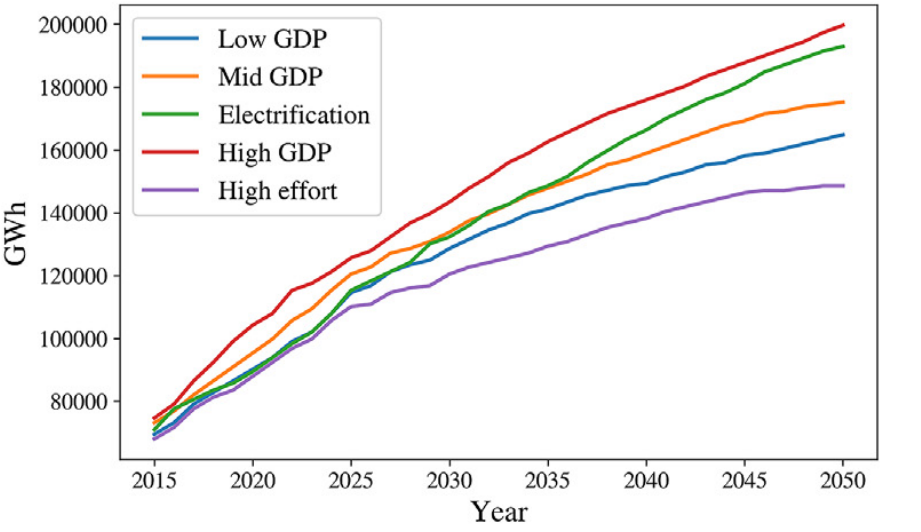
\includegraphics[width=8cm]{Submissions/EnergyPolicy/Images/demanda energetica segun escenario.png}
    \caption{{\footnotesize Demand scenarios.}}
    \label{fig:demandaescenarios}
\end{figure}

Each scenario is defined as ... 
% To print the credit authorship contribution details
%\printcredits

%% Loading bibliography style file
%\bibliographystyle{model1-num-names}
\bibliographystyle{cas-model2-names}

% Loading bibliography database
\bibliography{references}

% Biography
%\bio{}
% Here goes the biography details.
%\endbio

%\bio{pic1}
% Here goes the biography details.
%\endbio

\end{document}

